\documentclass[a4paper]{article}

\def\npart {IB}
\def\nterm {Easter}
\def\nyear {2015}
\def\nlecturer {J.\ Rasmussen}
\def\ncourse {Metric and Topological Spaces}

\usepackage{myheader}

\begin{document}
\maketitle
{\small
\noindent\textbf{Metrics}\\
Definition and examples. Limits and continuity. Open sets and neighbourhoods. Characterizing limits and continuity using neighbourhoods and open sets.\hspace*{\fill} [3]

\vspace{10pt}
\noindent\textbf{Topology}\\
Definition of a topology. Metric topologies. Further examples. Neighbourhoods, closed sets, convergence and continuity. Hausdorff spaces. Homeomorphisms. Topological and non-topological properties. Completeness. Subspace, quotient and product topologies.\hspace*{\fill} [3]

\vspace{10pt}
\noindent\textbf{Connectedness}\\
Definition using open sets and integer-valued functions. Examples, including intervals. Components. The continuous image of a connected space is connected. Path-connectedness. Path-connected spaces are connected but not conversely. Connected open sets in Euclidean space are path-connected.\hspace*{\fill} [3]

\vspace{10pt}
\noindent\textbf{Compactness}\\
Definition using open covers. Examples: finite sets and [0, 1]. Closed subsets of compact spaces are compact. Compact subsets of a Hausdorff space must be closed. The compact subsets of the real line. Continuous images of compact sets are compact. Quotient spaces. Continuous real-valued functions on a compact space are bounded and attain their bounds. The product of two compact spaces is compact. The compact subsets of Euclidean space. Sequential compactness.\hspace*{\fill} [3]}

\tableofcontents
\setcounter{section}{-1}
\section{Introduction}
The course \emph{Metric and Topological Spaces} is divided into two parts. The first is on metric spaces, and the second is on topological spaces (duh).

In Analysis, we studied real numbers a lot. We defined many properties such as convergence of sequences and continuity of functions. For example, if $(x_n)$ is a sequence in $\R$, $x_n \to x$ means
\[
  (\forall \varepsilon > 0)(\exists N)(\forall n > N)\, |x_n - x| < \varepsilon.
\]
Similarly, a function $f$ is continuous at $x_0$ if
\[
  (\forall \varepsilon > 0)(\exists \delta > 0)(\forall x)\,|x - x_0| < \delta \Rightarrow |f(x) - f(x_0)| < \varepsilon.
\]
However, the definition of convergence doesn't really rely on $x_n$ being real numbers, except when calculating values of $|x_n - x|$. But what does $|x_n - x|$ really mean? It is the distance between $x_n$ and $x$. To define convergence, we don't really need notions like subtraction and absolute values. We simply need a (sensible) notion of distance between points.

Given a set $X$, we can define a \emph{metric} (``distance function'') $d: X\times X\to \R$, where $d(x, y)$ is the distance between the points $x$ and $y$. Then we say a sequence $(x_n)$ in $X$ converges to $x$ if
\[
  (\forall \varepsilon > 0)(\exists N)(\forall n > N)\, d(x_n, x) < \varepsilon.
\]
Similarly, a function $f: X\to X$ is continuous if
\[
  (\forall \varepsilon > 0)(\exists \delta > 0)(\forall x)\,d(x, x_0) < \delta \Rightarrow d(f(x), f(x_0)) < \varepsilon.
\]
Of course, we will need the metric $d$ to satisfy certain conditions such as being non-negative, and we will explore these technical details in the first part of the course.

As people studied metric spaces, it soon became evident that metrics are not really that useful a notion. Given a set $X$, it is possible to find many different metrics that completely agree on which sequences converge and what functions are continuous.

It turns out that it is not the metric that determines (most of) the properties of the space. Instead, it is the \emph{open sets} induced by the metric (intuitively, an open set is a subset of $X$ without ``boundary'', like an open interval). Metrics that induce the same open sets will have almost identical properties (apart from the actual distance itself).

The idea of a topological space is to just keep the notion of open sets and abandon metric spaces, and this turns out to be a really good idea. The second part of the course is the study of these topological spaces and defining a lot of interesting properties just in terms of open sets.

\section{Metric spaces}
\subsection{Definitions}
As mentioned in the introduction, given a set $X$, it is often helpful to have a notion of distance between points. This distance function is known as the \emph{metric}.
\begin{defi}[Metric space]
  A \emph{metric space} is a pair $(X, d_X)$ where $X$ is a set (the \emph{space}) and $d_X$ is a function $d_X: X \times X \to \R$ (the \emph{metric}) such that for all $x, y, z$,
  \begin{itemize}
    \item $d_X(x, y) \geq 0$\hfill(non-negativity)
    \item $d_X(x, y) = 0$ iff $x = y$\hfill(identity of indiscernibles)
    \item $d_X(x, y) = d_X(y, x)$\hfill(symmetry)
    \item $d_X(x, z) \leq d_X(x, y) + d_X(y, z)$\hfill(triangle inequality)
  \end{itemize}
\end{defi}

We will have two quick examples of metrics before going into other important definitions. We will come to more examples afterwards.
\begin{eg}\leavevmode
  \begin{itemize}
    \item (Euclidean ``usual'' metric) Let $X = \R^n$. Let
      \[
        d(\mathbf{v}, \mathbf{w}) = |\mathbf{v} - \mathbf{w}| = \sqrt{\sum_{i = 1}^n (v_i - w_i)^2}.
      \]
      This is the usual notion of distance we have in the $\R^n$ vector space. It is not difficult to show that this is indeed a metric (the fourth axiom follows from the Cauchy-Schwarz inequality).
    \item (Discrete metric) Let $X$ be a set, and
      \[
        d_X(x, y) =
        \begin{cases}
          1 & x \not= y\\
          0 & x = y
        \end{cases}
      \]
      To show this is indeed a metric, we have to show it satisfies all the axioms. The first three axioms are trivially satisfied. How about the fourth? We can prove this by exhaustion.

      Since the distance function can only return $0$ or $1$, $d(x, z)$ can be $0$ or $1$, while $d(x, y) + d(y, z)$ can be $0$, $1$ or $2$. For the fourth axiom to fail, we must have RHS $<$ LHS. This can only happen if the right hand side is $0$. But for the right hand side to be $0$, we must have $x = y = z$. So the left hand side is also $0$. So the fourth axiom is always satisfied.
  \end{itemize}
\end{eg}

Given a metric space $(X, d)$, we can generate another metric space by picking out a subset of $X$ and reusing the same metric.
\begin{defi}[Metric subspace]
  Let $(X, d_X)$ be a metric space, and $Y\subseteq X$. Then $(Y, d_Y)$ is a metric space, where $d_Y(a, b) = d_X(a, b)$, and said to be a \emph{subspace} of $X$.
\end{defi}

\begin{eg}
  $S^n = \{\mathbf{v}\in \R^{n + 1}: |\mathbf{v}| = 1\}$, the $n$-dimensional sphere, is a subspace of $\R^{n + 1}$.
\end{eg}

Finally, as promised, we come to the definition of convergent sequences and continuous functions.
\begin{defi}[Convergent sequences]
  Let $(x_n)$ be a sequence in a metric space $(X, d_X)$. We say $(x_n)$ \emph{converges to} $x\in X$, written $x_n \to x$, if $d(x_n, x) \to 0$ (as a real sequence). Equivalently,
  \[
    (\forall \varepsilon > 0)(\exists N)(\forall n > N)\, d(x_n, x) < \varepsilon.
  \]
\end{defi}
\begin{eg}\leavevmode
  \begin{itemize}
    \item Let $(\mathbf{v}_n)$ be a sequence in $\R^k$ with the Euclidean metric. Write $\mathbf{v}_n = (v_n^1, \cdots, v_n^k)$, and $\mathbf{v} = (v^1, \cdots, v^k)\in \R^k$. Then $\mathbf{v}_n \to \mathbf{v}$ iff $(v_n^i) \to v^i$ for all $i$.

    \item Let $X$ have the discrete metric, and suppose $x_n \to x$. Pick $\varepsilon = \frac{1}{2}$. Then there is some $N$ such that $d(x_n, x) < \frac{1}{2}$ whenever $n > N$. But if $d(x_n, x) < \frac{1}{2}$, we must have $d(x_n, x) = 0$. So $x_n = x$. Hence if $x_n \to x$, then eventually all $x_n$ are equal to $x$.

  \end{itemize}
\end{eg}

Similar to what we did in Analysis, we can show that limits are unique (if exist).
\begin{prop}
  If $(X, d)$ is a metric space, $(x_n)$ is a sequence in $X$ such that $x_n \to x$, $x_n \to x'$, then $x = x'$.
\end{prop}

\begin{proof}
  For any $\varepsilon > 0$, we know that there exists $N$ such that $d(x_n, x) < \varepsilon/2$ if $n > N$. Similarly, there exists some $N'$ such that $d(x_n, x') < \varepsilon/2$ if $n > N'$.

  Hence if $n > \max(N, N')$, then
  \begin{align*}
    0 &\leq d(x, x')\\
    &\leq d(x, x_n) + d(x_n, x')\\
    &= d(x_n, x) + d(x_n, x')\\
    &\leq \varepsilon.
  \end{align*}
  So $0 \leq d(x, x') \leq \varepsilon$ for all $\varepsilon > 0$. So $d(x, x') = 0$, and $x = x'$.
\end{proof}

Note that to prove the above proposition, we used all of the four axioms. In the first line, we used non-negativity to say $0\leq d(x, x')$. In the second line, we used triangle inequality. In the third line, we used symmetry to swap $d(x, x_n)$ with $d(x_n, x)$. Finally, we used the identity of indiscernibles to conclude that $x = x'$.

To define a continuous function, here, we opt to use the sequence definition. We will later show that this is indeed equivalent to the $\varepsilon-\delta$ definition, as well as a few other more useful definitions.
\begin{defi}[Continuous function]
  Let $(X, d_X)$ and $(Y, d_Y)$ be metric spaces, and $f:X \to Y$. We say $f$ is \emph{continuous} if $f(x_n) \to f(x)$ (in $Y$) whenever $x_n \to x$ (in $X$).
\end{defi}

\begin{eg}
  Let $X = \R$ with the Euclidean metric. Let $Y = \R$ with the discrete metric. Then
  $f:X \to Y$ that maps $f(x) = x$ is not continuous. This is since $1/n \to 0$ in the Euclidean metric, but not in the discrete metric.

  On the other hand, $g: Y\to X$ by $g(x) = x$ is continuous, since a sequence in $Y$ that converges is eventually constant.
\end{eg}

\subsection{Examples of metric spaces}
In this section, we will give four different examples of metrics, where the first two are metrics on $\R^2$. There is an obvious generalization to $\R^n$, but we will look at $\R^2$ specifically for the sake of simplicity.
\begin{eg}[Manhattan metric]
  Let $X = \R^2$, and define the metric as
  \[
    d(\mathbf{x}, \mathbf{y}) = d((x_1, x_2), (y_1, y_2)) = |x_1 - y_1| + |x_2 - y_2|.
  \]
  The first three axioms are again trivial. To prove the triangle inequality, we have
  \begin{align*}
    d(\mathbf{x}, \mathbf{y}) + d(\mathbf{y}, \mathbf{z}) &= |x_1 - y_1| + |x_2 - y_2| + |y_1 - z_1| + |y_2 - z_2|\\
    &\geq |x_1 - z_1| + |z_2 - z_2|\\
    &= d(\mathbf{x}, \mathbf{z}),
  \end{align*}
  using the triangle inequality for $\R$.

  This metric represents the distance you have to walk from one point to another if you are only allowed to move horizontally and vertically (and not diagonally).
\end{eg}

\begin{eg}[British railway metric]
  Let $X = \R^2$. We define
  \[
    d(\mathbf{x}, \mathbf{y}) =
    \begin{cases}
      |\mathbf{x} - \mathbf{y}|&\text{if }\mathbf{x} = k\mathbf{y}\\
      |\mathbf{x}| + |\mathbf{y}|&\text{otherwise}
    \end{cases}
  \]
  To explain the name of this metric, think of Britain with London as the origin. Since the railway system is \st{stupid} less than ideal, all trains go through London. For example, if you want to go from Oxford to Cambridge (and obviously not the other way round), you first go from Oxford to London, then London to Cambridge. So the distance traveled is the distance from London to Oxford plus the distance from London to Cambridge.

  The exception is when the two destinations lie along the same line, in which case, you can directly take the train from one to the other without going through London, and hence the ``if $\mathbf{x} = k\mathbf{y}$'' clause.
\end{eg}

\begin{eg}[$p$-adic metric]
  Let $p\in \Z$ be a prime number. We first define the norm $|n|_p$ to be $p^{-k}$, where $k$ is the highest power of $p$ that divides $n$. If $n = 0$, we let $|n|_p = 0$. For example, $|20|_2 = |2^2\cdot 5|_2 = 2^{-2}$.

  Now take $X = \Z$, and let $d_p (a, b) = |a - b|_p$. The first three axioms are trivial, and the triangle inequality can be proved by making some number-theoretical arguments about divisibility.

  This metric has rather interesting properties. With respect to $d_2$, we have $1, 2, 4, 8, 16, 32, \cdots \to 0$, while $1, 2, 3, 4, \cdots$ does not converge. We can also use it to prove certain number-theoretical results, but we will not go into details here.
\end{eg}

\begin{eg}[Uniform metric]
  Let $X = C[0, 1]$ be the set of all continuous functions on $[0, 1]$. Then define
  \[
    d(f, g) = \max_{x\in [0, 1]}|f(x) - g(x)|.
  \]
  The maximum always exists since continuous functions on $[0, 1]$ are bounded and attain their bounds.

  Now let $F: C[0, 1] \to \R$ be defined by $F(f) = f(\frac{1}{2})$. Then this is continuous with respect to the uniform metric on $C[0, 1]$ and the usual metric on $\R$:

  Let $f_n \to f$ in the uniform metric. Then we have to show that $F(f_n) \to F(f)$, i.e.\ $f_n(\frac{1}{2}) \to f(\frac{1}{2})$. This is easy, since we have
  \[
    0 \leq |F(f_n) - F(f)| = |f_n(\tfrac{1}{2}) - f(\tfrac{1}{2})| \leq \max|f_n(x) - f(x)| \to 0.
  \]
  So $|f_n(\frac{1}{2}) - f(\frac{1}{2})| \to 0$. So $f_n(\frac{1}{2}) \to f(\frac{1}{2})$.
\end{eg}

\subsection{Norms}
There are several notions on vector spaces that are closely related to metrics. We'll look at \emph{norms} and \emph{inner products} of vector spaces, and show that they all naturally induce a metric on the space.

First of all, we define the norm. This can be thought of as the ``length'' of a vector in the vector space.
\begin{defi}[Norm]
  Let $V$ be a real vector space. A \emph{norm} on $V$ is a function $\|\ph \|: V\to \R$ such that
  \begin{itemize}
    \item $\|\mathbf{v}\| \geq 0$ for all $\mathbf{v}\in V$
    \item $\|\mathbf{v}\| = 0$ if and only if $\mathbf{v} = \mathbf{0}$.
    \item $\|\lambda \mathbf{v}\| = |\lambda|\|\mathbf{v}\|$
    \item $\|\mathbf{v} + \mathbf{w}\| \leq \|\mathbf{v}\| + \|\mathbf{w}\|$.
  \end{itemize}
\end{defi}

\begin{eg}
  Let $V = \R^n$. There are several possible norms we can define on $\R^n$:
  \begin{align*}
    \|\mathbf{v}\|_1 &= \sum_{i = 1}^n |v_i|\\
    \|\mathbf{v}\|_2 &= \sqrt{\sum_{i = 1}^n v_i^2}\\
    \|\mathbf{v}\|_\infty &= \max \{|v_i|: 1 \leq i \leq n\}.
  \end{align*}
  In general, we can define the norm
  \[
    \|\mathbf{v}\|_p = \left(\sum_{i = 1}^n |v_i|^p\right)^{1/p}.
  \]
  for any $1 \leq p \leq \infty$, and $\|\mathbf{v}\|_\infty$ is the limit as $p\to \infty$.

  Proof that these are indeed norms is left as an exercise for the reader (in the example sheets).
\end{eg}

A norm naturally induces a metric on $V$:
\begin{lemma}
  If $\|\ph\|$ is a norm on $V$, then
  \[
    d(\mathbf{v}, \mathbf{w}) = \|\mathbf{v} - \mathbf{w}\|
  \]
  defines a metric on $V$.
\end{lemma}

\begin{proof}\leavevmode
  \begin{enumerate}
    \item $d(\mathbf{v}, \mathbf{w}) = \|\mathbf{v} - \mathbf{w}\| \geq 0$ by the definition of the norm.
    \item $d(\mathbf{v}, \mathbf{w}) = 0 \Leftrightarrow \|\mathbf{v} - \mathbf{w}\| = 0 \Leftrightarrow \mathbf{v} - \mathbf{w} = \mathbf{0} \Leftrightarrow \mathbf{v} = \mathbf{w}$.
    \item $d(\mathbf{w}, \mathbf{v}) = \|\mathbf{w} - \mathbf{v}\| = \|(-1)(\mathbf{v} - \mathbf{w})\| = |-1| \|\mathbf{v} - \mathbf{w}\| = d(\mathbf{v}, \mathbf{w})$.
    \item $d(\mathbf{u}, \mathbf{v}) + d(\mathbf{v}, \mathbf{w}) = \|\mathbf{u} - \mathbf{v}\| + \|\mathbf{v} - \mathbf{w}\| \geq \|\mathbf{u} - \mathbf{w}\| = d(\mathbf{u}, \mathbf{w})$.\qedhere
  \end{enumerate}
\end{proof}

\begin{eg}
  We have the following norms on $C[0, 1]$:
  \begin{align*}
    \|f\|_1 &= \int_0^1 |f(x)|\;\d x\\
    \|f\|_2 &= \sqrt{\int_0^1 f(x)^2 \;\d x}\\
    \|f\|_{\infty} &= \max_{x \in [0, 1]}|f(x)|
  \end{align*}
  The first two are known as the $L^1$ and $L^2$ norms. The last is called the uniform norm, since it induces the uniform metric.
\end{eg}
It is easy to show that these are indeed norms. The only slightly tricky part is to show that $\|f\| = 0$ iff $f = 0$, which we obtain via the following lemma.

\begin{lemma}
  Let $f\in C[0, 1]$ satisfy $f(x) \geq 0$ for all $x\in [0, 1]$. If $f(x)$ is not constantly $0$, then $\int_0^1 f(x)\;\d x > 0$.
\end{lemma}

\begin{proof}
  Pick $x_0 \in [0, 1]$ with $f(x_0) = a > 0$. Then since $f$ is continuous, there is a $\delta$ such that $|f(x) - f(x_0)| < a/2$ if $|x - x_0| < \delta$. So $|f(x)| > a/2$ in this region.

  Take
  \[
    g(x) =
    \begin{cases}
      a/2 & |x - x_0| < \delta\\
      0 & \text{otherwise}
    \end{cases}
  \]
  Then $f(x) \geq g(x)$ for all $x\in [0, 1]$. So
  \[
    \int_0^1 f(x)\;\d x \geq \int_0^1 g(x)\;\d x = \frac{a}{2}\cdot (2\delta) > 0.\qedhere
  \]
\end{proof}

\begin{eg}
  Let $X = C[0, 1]$, and let
  \[
    d_1(f, g) = \|f - g\|_1 = \int_0^1 |f(x) - g(x)|\;\d x.
  \]
  Define the sequence
  \[
    f_n =
    \begin{cases}
      1 - nx & x \in [0, \frac{1}{n}]\\
      0 & x \geq \frac{1}{n}.
    \end{cases}
  \]
  \begin{center}
    \begin{tikzpicture}
      \draw [->] (-0.5, 0) -- (3, 0) node [above] {$f$};
      \draw [->] (0, -0.5) -- (0, 2) node [right] {$x$};
      \draw [red, thick] (0, 1.5) -- (0.5, 0) node [below, black] {$\frac{1}{n}$} -- (2, 0) node [below, black] {$1$};
    \end{tikzpicture}
  \end{center}
  Then
  \[
    \|f\|_1 = \frac{1}{2}\cdot \frac{1}{n} \cdot 1 = \frac{1}{2n} \to 0
  \]
  as $n \to \infty$. So $f_n \to 0$ in $(X, d_1)$ where $0(x) = 0$.

  On the other hand,
  \[
    \|f_n\|_\infty = \max_{x\in [0, 1]} \|f(x)\| = 1.
  \]
  So $f_n \not\to 0$ in the uniform metric.

  So the function $(C[0, 1], d_1) \to (C[0, 1], d_\infty)$ that maps $f\mapsto f$ is \emph{not} continuous. This is similar to the case that the identity function from the usual metric of $\R$ to the discrete metric of $\R$ is not continuous. However, the discrete metric is a \emph{silly} metric, but $d_1 $ is a genuine useful metric here.

  Using the same example, we can show that the function $G: (C[0, 1], d_1) \to (\R, \text{usual})$ with $G(f) = f(0)$ is not continuous.
\end{eg}

We'll now define the inner product of a real vector space. This is a generalization of the notion of the ``dot product''.
\begin{defi}[Inner product]
  Let $V$ be a real vector space. An \emph{inner product} on $V$ is a function $\bra \ph, \ph\ket: V\times V \to \R$ such that
  \begin{enumerate}
    \item $\bra \mathbf{v}, \mathbf{v}\ket \geq 0$ for all $\mathbf{v}\in V$
    \item $\bra \mathbf{v}, \mathbf{v}\ket = 0$ if and only if $\mathbf{v} = \mathbf{0}$.
    \item $\bra \mathbf{v}, \mathbf{w}\ket = \bra \mathbf{w}, \mathbf{v}\ket$.
    \item $\bra \mathbf{v}_1 + \lambda \mathbf{v}_2, \mathbf{w}) = \bra \mathbf{v}_1, \mathbf{w}\ket + \lambda\bra \mathbf{v}_2 , \mathbf{w}\ket$.
  \end{enumerate}
\end{defi}

\begin{eg}\leavevmode
  \begin{enumerate}
    \item Let $V = \R^n$. Then
      \[
        \bra \mathbf{v}, \mathbf{w} \ket = \sum_{i = 1}^n v_i w_i
      \]
      is an inner product.
    \item Let $V = C[0, 1]$. Then
      \[
        \bra f, g\ket = \int_0^1 f(x) g(x) \;\d x
      \]
      is an inner product.
  \end{enumerate}
\end{eg}

We just showed that norms induce metrics. The proof was completely trivial as the definitions were almost the same. Now we want to prove that inner products induce norms. However, this is slightly less trivial. To do so, we need the Cauchy-Schwarz inequality.

\begin{thm}[Cauchy-Schwarz inequality]
  If $\bra\ph,\ph\ket$ is an inner product, then
  \[
    \bra \mathbf{v}, \mathbf{w}\ket^2 \leq \bra \mathbf{v}, \mathbf{v}\ket\bra\mathbf{w},\mathbf{w}\ket.
  \]
\end{thm}

\begin{proof}
  For any $x$, we have
  \[
    \bra \mathbf{v} + x\mathbf{w}, \mathbf{v} + x \mathbf{w}\ket = \bra \mathbf{v}, \mathbf{v}\ket + 2x\bra \mathbf{v}, \mathbf{w}\ket + x^2 \bra \mathbf{w}, \mathbf{w}\ket \geq 0.
  \]
  Seen as a quadratic in $x$, since it is always non-negative, it can have at most one real root. So
  \[
    (2 \bra \mathbf{v}, \mathbf{w}\ket)^2 - 4\bra \mathbf{v}, \mathbf{v}\ket \bra \mathbf{w}, \mathbf{w}\ket \leq 0.
  \]
  So the result follows.
\end{proof}

With this, we can show that inner products induce norms (and hence metrics).
\begin{lemma}
  If $\bra \ph, \ph \ket$ is an inner product on $V$, then
  \[
    \|\mathbf{v}\| = \sqrt{\bra \mathbf{v}, \mathbf{v}\ket}
  \]
  is a norm.
\end{lemma}

\begin{proof}\leavevmode
  \begin{enumerate}
    \item $\|\mathbf{v}\| = \sqrt{\bra \mathbf{v}, \mathbf{v}\ket} \geq 0$.
    \item $\|\mathbf{v}\| = 0\Leftrightarrow \bra \mathbf{v}, \mathbf{v}\ket = 0 \Leftrightarrow \mathbf{v} = \mathbf{0}$.
    \item $\|\lambda \mathbf{v}\| = \sqrt{\bra \lambda \mathbf{v}, \lambda \mathbf{v}\ket} = \sqrt{\lambda^2 \bra \mathbf{v}, \mathbf{v}\ket} = |\lambda| \|\mathbf{v}\|$.
    \item
      \begin{align*}
        (\|\mathbf{v}\| + \|\mathbf{w}\|)^2 &= \|\mathbf{v}\|^2 + 2\|\mathbf{v}\|\|\mathbf{w}\| + \|\mathbf{w}\|^2\\
        &\geq \bra \mathbf{v}, \mathbf{v}\ket + 2\bra \mathbf{v}, \mathbf{w}\ket + \bra \mathbf{w}, \mathbf{w}\ket \\
        &= \|\mathbf{v} + \mathbf{w}\|^2\qedhere
      \end{align*}%\qedhere
  \end{enumerate}
\end{proof}

\subsection{Open and closed subsets}
In this section, we will study open and closed subsets of metric spaces. We will then proceed to prove certain key properties of open and closed subsets, and show that they are all we need to define continuity. This will lead to the next chapter (and the rest of the course), where we completely abandon the idea of metrics and only talk about open and closed subsets.

To define open and closed subsets, we first need the notion of balls.
\begin{defi}[Open and closed balls]
  Let $(X, d)$ be a metric space. For any $x\in X$, $r\in \R$,
  \[
    B_r(x) = \{y\in X: d(y, x) < r\}
  \]
  is the \emph{open ball} centered at $x$.
  \[
    \bar{B}_r(x) = \{y\in X: d(y, x) \leq r\}
  \]
  is the \emph{closed ball} centered at $x$.
\end{defi}

\begin{eg}\leavevmode
  \begin{enumerate}
    \item When $X = \R$, $B_r(x) = (x - r, x + r)$. $\bar{B}_r(x) = [x - r, x + r]$.
    \item When $X = \R^2$,
      \begin{enumerate}
        \item If $d$ is the metric induced by the $\|\mathbf{v}\|_1 = |v_1| + |v_2|$, then an open ball is a rotated square.
          \begin{center}
            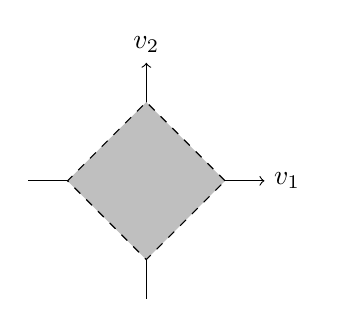
\begin{tikzpicture}
              \draw [->] (-1.5, 0) -- (1.5, 0) node [right] {$v_1$};
              \draw [->] (0, -1.5) -- (0, 1.5) node [above] {$v_2$};
              \draw [dashed, fill=gray!50!white] (1, 0) -- (0, 1) -- (-1, 0) -- (0, -1) --cycle;
            \end{tikzpicture}
          \end{center}
        \item If $d$ is the metric induced by the $\|\mathbf{v}\|_2 = \sqrt{v_1^2 + v_2^2}$, then an open ball is an actual disk.
          \begin{center}
            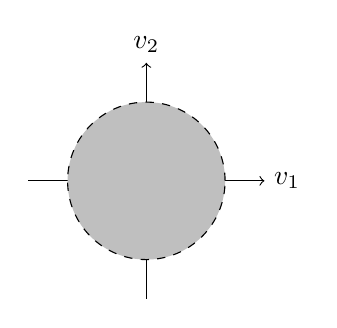
\begin{tikzpicture}
              \draw [->] (-1.5, 0) -- (1.5, 0) node [right] {$v_1$};
              \draw [->] (0, -1.5) -- (0, 1.5) node [above] {$v_2$};
              \draw [dashed, fill=gray!50!white] circle [radius=1];
            \end{tikzpicture}
          \end{center}

        \item If $d$ is the metric induced by the $\|\mathbf{v}\|_\infty = \max\{|v_1|, |v_2|\}$, then an open ball is a square.
          \begin{center}
            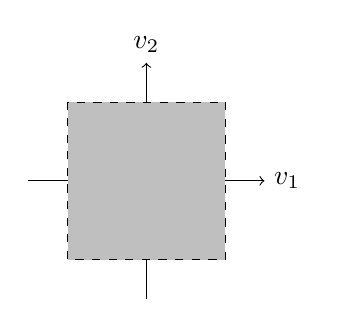
\begin{tikzpicture}
              \draw [->] (-1.5, 0) -- (1.5, 0) node [right] {$v_1$};
              \draw [->] (0, -1.5) -- (0, 1.5) node [above] {$v_2$};
              \draw [dashed, fill=gray!50!white] (1, 1) -- (1, -1) -- (-1, -1) -- (-1, 1) --cycle;
            \end{tikzpicture}
          \end{center}
      \end{enumerate}
  \end{enumerate}
\end{eg}
\begin{defi}[Open subset]
  $U\subseteq X$ is an \emph{open subset} if for every $x\in U$, $\exists \delta > 0$ such that $B_\delta(x) \subseteq U$.

  $C\subseteq X$ is a \emph{closed subset} if $X\setminus C \subseteq X$ is open.
\end{defi}
As if we've not emphasized this enough, this is a very \emph{very} important definition.

We first prove that this is a sensible definition.
\begin{lemma}
  The open ball $B_r(x) \subseteq X$ is an open subset, and the closed ball $\bar{B}_r(x) \subseteq X$ is a closed subset.
\end{lemma}

\begin{proof}
  Given $y\in B_r(x)$, we must find $\delta > 0$ with $B_\delta(y) \subseteq B_r(x)$.
  \begin{center}
    \begin{tikzpicture}
      \draw [->] (-1.5, 0) -- (1.5, 0) node [right] {$v_1$};
      \draw [->] (0, -1.5) -- (0, 1.5) node [above] {$v_2$};
      \draw [dashed, fill=gray!50!white] circle [radius=1];
      \draw (0, 0) -- (0.707, 0.707) node [below, pos = 0.5] {$r$};
      \draw (0.5, 0.5) node [circ] {} node [right] {$y$};
      \draw [dashed] (0.5, 0.5) circle [radius=0.293];
    \end{tikzpicture}
  \end{center}
  Since $y\in B_r(x)$, we must have $a = d(y, x) < r$. Let $\delta = r - a > 0$. Then if $z \in B_\delta (y)$, then
  \[
    d(z, x)\leq d(z, y) + d(y, x) < (r - a) + a = r.
  \]
  So $z \in B_r(x)$. So $B_r(y) \subseteq B_r(x)$ as desired.

  The second statement is equivalent to $X\setminus \bar{B}_r(x) = \{y\in X: d(y, x) > r\}$ is open. The proof is very similar.
\end{proof}
Note that openness is a property of a \emph{subset}. $A\subseteq X$ being open depends on both $A$ and $X$, not just $A$. For example, $[0, \frac{1}{2})$ is not an open subset of $\R$, but is an open subset of $[0, 1]$ (since it is $B_{\frac{1}{2}}(0)$), both with the Euclidean metric. However, we are often lazy and just say ``open set'' instead of ``open subset''.

\begin{eg}\leavevmode
  \begin{enumerate}
    \item $(0, 1)\subseteq \R$ is open, while $[0, 1]\subseteq \R$ is closed. $[0, 1)\subseteq \R$ is neither closed nor open.
    \item $\Q\subseteq \R$ is neither open nor closed, since any open interval contains both rational numbers and irrational numbers. So any open interval cannot be a subset of $\Q$ or $\R\setminus \Q$.
    \item Let $X = [-1, 1] \setminus \{0\}$ with the Euclidean metric. Let $A = [-1, 0)\subseteq X$. Then $A$ is open since it is equal to $B_1(-1)$. $A$ is also closed since it is equal to $\bar B_{\frac{1}{2}}(-\frac{1}{2})$.
  \end{enumerate}
\end{eg}

\begin{defi}[Open neighborhood]
  If $x\in X$, an \emph{open neighborhood} of $x$ is an open $U\subseteq X$ with $x\in U$.
\end{defi}
This is not really an interesting definition, but is simply a convenient shorthand for ``open subset containing $x$''.

\begin{lemma}
  If $U$ is an open neighbourhood of $x$ and $x_n \to x$, then $\exists N$ such that $x_n \in U$ for all $n > N$.
\end{lemma}

\begin{proof}
  Since $U$ is open, there exists some $\delta > 0$ such that $B_\delta(x)\subseteq U$. Since $x_n \to x$, $\exists N$ such that $d(x_n, x) < \delta$ for all $n > N$. This implies that $x_n \in B_\delta(x)$ for all $n > N$. So $x_n \in U$ for all $n > N$.
\end{proof}

\begin{defi}[Limit point]
  Let $A\subseteq X$. Then $x\in X$ is a \emph{limit point} of $A$ if there is a sequence $x_n \to x$ such that $x_n \in A$ for all $n$.
\end{defi}
Intuitively, a limit point is a point we can get arbitrarily close to.

\begin{eg}\leavevmode
  \begin{enumerate}
    \item If $a\in A$, then $a$ is a limit point of $A$, by taking the sequence $a, a, a, a, \cdots$.
    \item If $A = (0, 1)\subseteq \R$, then $0$ is a limit point of $A$, e.g.\ take $x_n = \frac{1}{n}$.
    \item Every $x\in \R$ is a limit point of $\Q$.
  \end{enumerate}
\end{eg}

It is possible to characterize closed subsets by limit points. This is often a convenient way of proving that sets are closed.
\begin{prop}
  $C\subseteq X$ is a closed subset if and only if every limit point of $C$ is an element of $C$.
\end{prop}

\begin{proof}
  $(\Rightarrow)$ Suppose $C$ is closed and $x_n \to x$, $x_n \in C$. We have to show that $x\in C$.

  Since $C$ is closed, $A = X\setminus C\subseteq X$ is open. Suppose the contrary that $x\not\in C$. Then $x\in A$. Hence $A$ is an open neighbourhood of $x$. Then by our previous lemma, we know that there is some $N$ such that $x_n \in A$ for all $n \geq N$. So $x_N \in A$. But we know that $x_N \in C$ by assumption. This is a contradiction. So we must have $x\in C$.

  $(\Leftarrow)$ Suppose that $C$ is not closed. We have to find a limit point not in $C$.

  Since $C$ is not closed, $A$ is not open. So $\exists x\in A$ such that $B_\delta(x)\not\subseteq A$ for all $\delta > 0$. This means that $B_\delta(x) \cap C \not= \emptyset$ for all $\delta > 0$.

  So pick $x_n \in B_{\frac{1}{n}}(x)\cap C$ for each $n > 0$. Then $x_n \in C$, $d(x_n, x) = \frac{1}{n} \to 0$. So $x_n \to x$. So $x$ is a limit point of $C$ which is not in $C$.
\end{proof}

Finally, we get to the Really Important Result\textsuperscript{TM} that tells us metrics are useless.
\begin{prop}[Characterization of continuity]
  Let $(X, d_x)$ and $(Y, d_y)$ be metric spaces, and $f: X\to Y$. The following conditions are equivalent:
  \begin{enumerate}
    \item $f$ is continuous
    \item If $x_n \to x$, then $f(x_n) \to f(x)$ (which is the definition of continuity)
    \item For any closed subset $C\subseteq Y$, $f^{-1}(C)$ is closed in $X$.
    \item For any open subset $U\subseteq Y$, $f^{-1}(U)$ is open in $X$.
    \item For any $x\in X$ and $\varepsilon > 0$, $\exists \delta > 0$ such that $f(B_\delta(x)) \subseteq B_\varepsilon(f(x))$. Alternatively, $d_x(x, z) < \delta \Rightarrow d_y(f(x), f(z)) < \varepsilon$.
  \end{enumerate}
\end{prop}

\begin{proof}\leavevmode
  \begin{itemize}
    \item $1 \Leftrightarrow 2$: by definition
    \item $2 \Rightarrow 3$: Suppose $C\subseteq Y$ is closed. We want to show that $f^{-1}(C)$ is closed. So let $x_n \to x$, where $x_n \in f^{-1}(C)$.

      We know that $f(x_n) \to f(x)$ by (2) and $f(x_n) \in C$. So $f(x)$ is a limit point of $C$. Since $C$ is closed, $f(x) \in C$. So $x\in f^{-1}(C)$. So every limit point of $f^{-1}(C)$ is in $f^{-1}(C)$. So $f^{-1}(C)$ is closed.
    \item $3 \Rightarrow 4$: If $U\subseteq Y$ is open, then $Y\setminus U$ is closed in Y. So $f^{-1}(Y\setminus U) = X\setminus f^{-1}(U)$ is closed in $X$. So $f^{-1}(U)\subseteq X$ is open.

    \item $4 \Rightarrow 5$: Given $x\in X, \varepsilon > 0$, $B_\varepsilon(f(x))$ is open in $Y$. By (4), we know $f^{-1}(B_\varepsilon(f(x))) = A$ is open in $X$. Since $x\in A$, $\exists \delta > 0$ with $B_\delta (x) \subseteq A$. So
      \[
        f(B_\delta(x)) \subseteq f(A) = f(f^{-1}(B_\varepsilon (f(x)))) = B_\varepsilon (f(x))
      \]
    \item $5 \Rightarrow 2$: Suppose $x_n \to x$. Given $\varepsilon > 0$, $\exists \delta > 0$ such that $f(B_\delta(x)) \subseteq B_\varepsilon(f(x))$. Since $x_n \to x$, $\exists N$ such that $x_n \in B_\delta (x)$ for all $n > N$. Then $f(x_n) \in f(B_\delta(x))\subseteq B_\varepsilon(f(x))$ for all $n > N$. So $f(x_n) \to f(x)$.\qedhere
  \end{itemize}
\end{proof}

The third and fourth condition can allow us to immediately decide if a subset is open or closed in some cases.

\begin{eg}
  Let $f: \R^3 \to \R$ be defined as
  \[
    f(x_1, x_2, x_3) = x_1^2 + x_2^4 x_3^6 + x_1^8 x_3^2.
  \]
  Then this is continuous. So $\{\mathbf{x}\in \R^3: f(\mathbf{x}) \leq 1\} = f^{-1}((-\infty, 1])$ is closed in $\R^3$.
\end{eg}

Before we end, we prove some key properties of open subsets. These will be used as the defining properties of open subsets in the next chapter.
\begin{lemma}\leavevmode
  \begin{enumerate}
    \item $\emptyset$ and $X$ are open subsets of $X$.
    \item Suppose $V_\alpha \subseteq X$ is open for all $\alpha \in A$. Then $\displaystyle U = \bigcup_{\alpha \in A}V_\alpha$ is open in $X$.
    \item If $V_1, \cdots, V_n\subseteq X$ are open, then so is $\displaystyle V = \bigcap_{i = 1}^n V_i$.
  \end{enumerate}
\end{lemma}

\begin{proof}\leavevmode
  \begin{enumerate}
    \item $\emptyset$ satisfies the definition of an open subset vacuously. $X$ is open since for any $x$, $B_1(x) \subseteq X$.
    \item If $x\in U$, then $x\in V_\alpha$ for some $\alpha$. Since $V_\alpha$ is open, there exists $\delta > 0$ such that $B_\delta(x) \subseteq V_\alpha$. So $\displaystyle B_\delta (x) \subseteq \bigcup_{\alpha \in A}V_\alpha = U$. So $U$ is open.
    \item If $x\in V$, then $x\in V_i$ for all $i = 1, \cdots, n$. So $\exists \delta_i > 0$ with $B_{\delta_i}(x) \subseteq V_i$. Take $\delta = \min\{\delta_1, \cdots, \delta_n\}$. So $B_\delta(x) \subseteq V_i$ for all $i$. So $B_\delta(x) \subseteq V$. So $V$ is open.\qedhere
  \end{enumerate}
\end{proof}
Note that we can take infinite unions or finite intersection, but not infinite intersections. For example, the intersection of all $(-\frac{1}{n}, \frac{1}{n})$ is $\{0\}$, which is not open.

\section{Topological spaces}
\subsection{Definitions}
We have previously shown that a function $f$ is continuous iff $f^{-1}(U)$ is open whenever $U$ is open. Convergence can also be characterized using open sets only. This suggests that we can dump the metric and just focus on the open sets.

What we will do is to define the \emph{topology} of a space $X$ to be the set of open sets of $X$. Then this topology would define most of the structure or geometry of $X$, and we don't need to care about metrics.

\begin{defi}[Topological space]
  A \emph{topological space} is a set $X$ (the space) together with a set $\cU \subseteq \P(X)$ (the topology) such that:
  \begin{enumerate}
    \item $\emptyset, X\in \cU$
    \item If $V_\alpha\in \cU$ for all $\alpha \in A$, then $\displaystyle \bigcup_{\alpha\in A}V_\alpha \in \cU$.
    \item If $V_1, \cdots, V_n \in \cU$, then $\displaystyle \bigcap_{i = 1}^n V_i \in \cU$.
  \end{enumerate}
  The elements of $X$ are the \emph{points}, and the elements of $\cU$ are the open subsets of $X$.
\end{defi}

\begin{defi}[Induced topology]
  Let $(X, d)$ be a metric space. Then the topology \emph{induced by} $d$ is the set of all open sets of $X$ under $d$.
\end{defi}

\begin{eg}
  Let $X = \R^n$ and consider the two metrics $d_1(\mathbf{x}, \mathbf{y}) = \|\mathbf{x} - \mathbf{y}\|_1$ and $d_\infty(\mathbf{x}, \mathbf{y}) = \|\mathbf{x} - \mathbf{y}\|_\infty$. We will show that they induce the same topology.

  Recall that the metrics are defined by
  \[
    \|\mathbf{v}\| = \sum_{i = 1}^n |v_i|,\quad \|\mathbf{v}\|_\infty = \max_{1 \leq i \leq n}|v_i|.
  \]
  This implies that
  \[
    \|\mathbf{v}\|_\infty \leq \|\mathbf{v}\|_1 \leq n\|\mathbf{v}\|_\infty.
  \]
  This in turn implies that
  \[
    B_r^\infty(x) \supseteq B_r^1 (x) \supseteq B_{r/n}^\infty(x).
  \]
  \begin{center}
    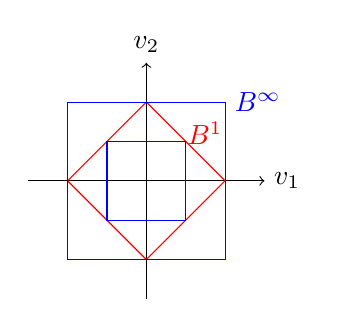
\begin{tikzpicture}
      \draw [->] (-1.5, 0) -- (1.5, 0) node [right] {$v_1$};
      \draw [->] (0, -1.5) -- (0, 1.5) node [above] {$v_2$};
      \draw [red] (1, 0) -- (0, 1) node [pos=0.6, right] {$B^1$} -- (-1, 0) -- (0, -1) -- cycle;
      \draw [blue] (1, 1) -- (1, -1) -- (-1, -1) -- (-1, 1) -- cycle node [right] {$B^{\infty}$};
      \draw [blue] (0.5, 0.5) -- (0.5, -0.5) -- (-0.5, -0.5) -- (-0.5, 0.5) -- cycle;
    \end{tikzpicture}
  \end{center}
  To show that the metrics induce the same topology, suppose that $U$ is open with respect to $d_1$, and we show that it is open with respect to $d_\infty$. Let $x \in U$. Since $U$ is open with respect to $d_1$, there exists some $\delta > 0$ such that $B_\delta^1(x)\subseteq U$. So $B_{\delta/n}^\infty (x) \subseteq B_\delta^1(x) \subseteq U$. So $U$ is open with respect to $d_\infty$.

  The other direction is similar.
\end{eg}

\begin{eg}
  Let $X = C[0, 1]$. Let $d_1(f, g) = \|f - g\|_1$ and $d_\infty(f, g) = \|f - g\|_\infty$. Then they do not induce the same topology, since $(X, d_1) \to (X, d_\infty)$ by $f\mapsto f$ is not continuous.
\end{eg}

It is possible to have some other topologies that are not induced by metrics.
\begin{eg}\leavevmode
  \begin{enumerate}
    \item Let $X$ be any set.
      \begin{enumerate}
        \item $\cU = \{\emptyset, X\}$ is the \emph{coarse topology} on $X$.
        \item $\cU = \P(X)$ is the \emph{discrete topology} on $X$, since it is induced by the discrete metric.
        \item $\cU = \{A\subseteq X: X\setminus A\text{ is finite or } A = \emptyset\}$ is the \emph{cofinite topology} on $X$.
      \end{enumerate}
    \item Let $X = \R$, and $\cU = \{(a, \infty): a\in \R\}$ is the \emph{right order topology} on $\R$.
  \end{enumerate}
\end{eg}

Now we can define continuous functions in terms of the topology only.
\begin{defi}[Continuous function]
  Let $f: X\to Y$ be a map of topological spaces. Then $f$ is \emph{continuous} if $f^{-1}(U)$ is open in $X$ whenever $U$ is open in $Y$.
\end{defi}
When the topologies are induced by metrics, the topological and metric notions of continuous functions coincide, as we showed in the previous chapter.

\begin{eg}\leavevmode
  \begin{enumerate}
    \item Any function $f: X\to Y$ is continuous if $X$ has the discrete topology.
    \item Any function $f: X\to Y$ is continuous if $Y$ has the coarse topology.
    \item If $X$ and $Y$ both have cofinite topology, then $f: X\to Y$ is continuous iff $f^{-1}(\{y\})$ is finite for every $y\in Y$.
  \end{enumerate}
\end{eg}

\begin{lemma}
  If $f: X\to Y$ and $g: Y\to Z$ are continuous, then so is $g\circ f: X\to Z$.
\end{lemma}

\begin{proof}
  If $U\subseteq Z$ is open, $g$ is continuous, then $g^{-1}(U)$ is open in $Y$. Since $f$ is also continuous, $f^{-1}(g^{-1}(U)) = (g\circ f)^{-1}(U)$ is open in $X$.
\end{proof}

In group theory, we had the notion of isomorphisms between groups. Isomorphic groups are equal-up-to-renaming-of-elements, and are considered to be the same for most purposes.

Similarly, we will define \emph{homeomorphisms} between topological spaces, and homeomorphic topological spaces will be considered to be the same (notice the ``e'' in hom\textbf{e}omorphism).
\begin{defi}[Homeomorphism]
  $f: X\to Y$ is a \emph{homeomorphism} if
  \begin{enumerate}
    \item $f$ is a bijection
    \item Both $f$ and $f^{-1}$ are continuous
  \end{enumerate}
  Equivalently, $f$ is a bijection and $U\subseteq X$ is open iff $f(U)\subseteq Y$ is open.

  Two spaces are \emph{homeomorphic} if there exists a homeomorphism between them, and we write $X\simeq Y$.
\end{defi}
Note that we specifically require $f$ and $f^{-1}$ to be both continuous. In group theory, if $\phi$ is a bijective homomorphism, then $\phi^{-1}$ is automatically a homomorphism as well. However, this is not true for topological spaces. $f$ being continuous does not imply $f^{-1}$ is continuous, as illustrated by the example below.

\begin{eg}
  Let $X = C[0, 1]$ with the topology induced by $\|\ph \|_1$ and $Y = C[0, 1]$ with the topology induced by $\|\ph\|_\infty$. Then $F: Y\to X$ by $f\mapsto f$ is continuous but $F^{-1}$ is not.
\end{eg}

\begin{eg}
  Let $X = [0, 2\pi)$ and $Y = S^1 = \{z \in \C: |z| = 1\}$. Then $f: X \to Y$ given by $f(x) = e^{ix}$ is continuous but its inverse is not.
\end{eg}

Similar to isomorphisms, we can show that homeomorphism is an equivalence relation.
\begin{lemma}
  Homeomorphism is an equivalence relation.
\end{lemma}

\begin{proof}\leavevmode
  \begin{enumerate}
    \item The identity map $I_X: X\to X$ is always a homeomorphism. So $X\simeq X$.
    \item If $f: X\to Y$ is a homeomorphism, then so is $f^{-1}:Y\to X$. So $X\simeq Y \Rightarrow Y\simeq X$.
    \item If $f: X\to Y$ and $g: Y\to Z$ are homeomorphisms, then $g\circ f: X\to Z$ is a homeomorphism. So $X\simeq Y$ and $Y\simeq Z$ implies $X\simeq Z$.\qedhere
  \end{enumerate}
\end{proof}

\begin{eg}\leavevmode
  \begin{enumerate}
    \item Under the usual topology, the open intervals $(0, 1)\simeq (a, b)$ for all $a, b\in \R$, using the homeomorphism $x\mapsto a + (b - a)x$.

      Similarly, $[0, 1] \simeq [a, b]$
    \item $(-1, 1) \simeq \R$ by $x\mapsto \tan(\frac{\pi}{2}x)$.
    \item $\R\simeq (0, \infty)$ by $x\mapsto e^x$.
    \item $(a, \infty)\simeq (b, \infty)$ by $x\mapsto x + (b - a)$.
  \end{enumerate}
  The fact that $\simeq$ is an equivalence relation implies that any 2 open intervals in $\R$ are homeomorphic.

\end{eg}
It is relatively easy to show that two spaces are homeomorphic. We just have to write down a homeomorphism. However, it is rather difficult to prove that two spaces are \emph{not homeomorphic}.

For example, is $(0, 1)$ homeomorphic to $[0, 1]$? No, but we aren't able to immediately prove it now. How about $\R$ and $\R^2$? Again they are not homeomorphic, but to show this we will need some tools that we'll develop in the next few lectures.

How about $\R^m$ and $\R^n$ in general? They are not homeomorphic, but we won't be able to prove this rigorously in the course. To properly prove this, we will need tools from algebraic topology.

So how can we prove that two spaces are not homeomorphic? In group theory, we could prove that two groups are not isomorphic by, say, showing that they have different orders. Similarly, to distinguish between topological spaces, we have to define certain \emph{topological properties}. Then if two spaces have different topological properties, we can show that they are not homeomorphic.

But before that, we will first define many many useful definitions in topological spaces, including sequences, subspaces, products and quotients. The remainder of the chapter will be mostly definitions that we will use later.
\subsection{Sequences}
To define the convergence of a sequence using open sets, we again need the concept of open neighbourhoods.

\begin{defi}[Open neighbourhood]
  An \emph{open neighbourhood} of $x\in X$ is an open set $U\subseteq X$ with $x\in U$.
\end{defi}

Now we can use this to define convergence of sequences.
\begin{defi}[Convergent sequence]
  A sequence $x_n \to x$ if for every open neighbourhood $U$ of $x$, $\exists N$ such that $x_n \in U$ for all $n > N$.
\end{defi}

\begin{eg}\leavevmode
  \begin{enumerate}
    \item If $X$ has the coarse topology, then any sequence $x_n$ converges to every $x\in X$, since there is only one open neighbourhood of $x$.
    \item If $X$ has the cofinite topology, no two $x_n$s are the same, then $x_n \to x$ for every $x\in X$, since every open set can only have finitely many $x_n$ not inside it.
  \end{enumerate}
\end{eg}

This looks weird. This is definitely not what we used to think of sequences. At least, we would want to have unique limits.

Fortunately, there is a particular class of spaces where sequences are well-behaved and have at most one limit.
\begin{defi}[Hausdorff space]
  A topological space $X$ is \emph{Hausdorff} if for all $x_1, x_2\in X$ with $x_1 \not= x_2$, there exist open neighbourhoods $U_1$ of $x_1$, $U_2$ of $x_2$ such that $U_1 \cap U_2 = \emptyset$.
\end{defi}

\begin{lemma}
  If $X$ is Hausdorff, $x_n$ is a sequence in $X$ with $x_n \to x$ and $x_n \to x'$, then $x = x'$, i.e.\ limits are unique.
\end{lemma}

\begin{proof}
  Suppose the contrary that $x\not= x'$. Then by definition of Hausdorff, there exist open neighbourhoods $U, U'$ of $x, x'$ respectively with $U \cap U' = \emptyset$.

  Since $x_n \to x$ and $U$ is a neighbourhood of $x$, by definition, there is some $N$ such that whenever $n > N$, we have $x_n \in U$. Similarly, since $x_n \to x'$, there is some $N'$ such that whenever $n > N'$, we have $x_n \in U'$.

  This means that whenever $n > \max(N, N')$, we have $x_n \in U$ and $x_n \in U'$. So $x_n \in U\cap U'$. This contradicts the fact that $U \cap U' = \emptyset$.

  Hence we must have $x = x'$.
\end{proof}

\begin{eg}\leavevmode
  \begin{enumerate}
    \item If $X$ has more than 1 element, then the coarse topology on $X$ is not Hausdorff.
    \item If $X$ has infinitely many elements, the cofinite topology on $X$ is not Hausdorff.
    \item The discrete topology is always Hausdorff.
    \item If $(X, d)$ is a metric space, the topology induced by $d$ is Hausdorff: for $x_1 \not= x_2$, let $r = d(x_1, x_2) > 0$. Then take $U_i = B_{r/2}(x_i)$. Then $U_1 \cap U_2 = \emptyset$.
  \end{enumerate}
\end{eg}

\subsection{Closed sets}
We will define closed sets similarly to what we did for metric spaces.

\begin{defi}[Closed sets]
  $C\subseteq X$ is \emph{closed} if $X\setminus C$ is an open subset of $X$.
\end{defi}

\begin{lemma}\leavevmode
  \begin{enumerate}
    \item If $C_\alpha$ is a closed subset of $X$ for all $\alpha \in A$, then $\bigcap_{\alpha \in A} C_\alpha$ is closed in $X$.
    \item If $C_1, \cdots, C_n$ are closed in $X$, then so is $\bigcup_{i = 1}^n C_i$.
  \end{enumerate}
\end{lemma}

\begin{proof}\leavevmode
  \begin{enumerate}
    \item Since $C_\alpha$ is closed in $X$, $X \setminus C_\alpha$ is open in $X$. So $\bigcup_{\alpha\in A}(X\setminus C_\alpha) = X\setminus \bigcap_{\alpha\in A}C_\alpha$ is open. So $\bigcap_{\alpha \in A}C_\alpha$ is closed.

    \item If $C_i$ is closed in $X$, then $X\setminus C_i$ is open. So $\bigcap_{i = 1}^n (X\setminus C_i) = X\setminus \bigcup_{i = 1}^n C_i$ is open. So $\bigcup_{i = 1}^n C_i$ is closed.\qedhere
  \end{enumerate}
\end{proof}

This time we can take infinite intersections and finite unions, which is the opposite of what we have for open sets.

Note that it is entirely possible to define the topology to be the collection of all \emph{closed} sets instead of open sets, but people seem to like open sets more.

\begin{cor}
  If $X$ is Hausdorff and $x\in X$, then $\{x\}$ is closed in $X$.
\end{cor}

\begin{proof}
  For all $y\in X$, there exist open subsets $U_y, V_y$ with $y\in U_y, x\in V_y$, $U_y \cap V_y = \emptyset$.

  Let $C_y = X\setminus U_y$. Then $C_y$ is closed, $y\not\in C_y$, $x\in C_y$. So $\{x\} = \bigcap_{y\not= x} C_y$ is closed since it is an intersection of closed subsets.
\end{proof}
\subsection{Closure and interior}
\subsubsection{Closure}
Given a subset $A\subseteq X$, if $A$ is not closed, we would like to find the smallest closed subset containing $A$. This is known as the \emph{closure} of $A$.

Officially, we define the closure as follows:

\begin{defi}
  Let $X$ be a topological space and $A\subseteq X$. Define
  \[
    \mathcal{C}_A = \{C\subseteq X: A\subseteq C\text{ and }C\text{ is closed in }X\}
  \]
  Then the \emph{closure} of $A$ in $X$ is
  \[
    \bar A = \bigcap_{C\in \mathcal{C}_A} C.
  \]
\end{defi}
First we do a sanity check: since $\bar A$ is defined as an intersection, we should make sure we are not taking an intersection of no sets. This is easy: since $X$ is closed in $X$ (its complement $\emptyset$ is open), $\mathcal{C}_A \not= \emptyset$. So we can safely take the intersection.

Since $\bar A$ is an intersection of closed sets, it is closed in $X$. Also, if $C\in \mathcal{C}_A$, then $A\subseteq C$. So $A\subseteq \bigcap_{C\in \mathcal{C}_A} C = \bar A$. In fact, we have

\begin{prop}
  $\bar A$ is the smallest closed subset of $X$ which contains $A$.
\end{prop}

\begin{proof}
  Let $K\subseteq X$ be a closed set containing $A$. Then $K\in \mathcal{C}_A$. So $\bar A = \bigcap_{C\in \mathcal{C}_A}C \subseteq K$. So $\bar A\subseteq K$.
\end{proof}

We basically \emph{defined} the closure such that it is the smallest closed subset of $X$ which contains $A$.

However, while this ``clever'' definition makes it easy to prove the above property, it is rather difficult to directly use it to compute the closure.

To compute the closure, we define the \emph{limit point} analogous to what we did for metric spaces.
\begin{defi}[Limit point]
  A \emph{limit point} of $A$ is an $x\in X$ such that there is a sequence $x_n \to x$ with $x_n \in A$ for all $n$.
\end{defi}
In general, limit points are easier to compute, and can be a useful tool for determining the closure of $A$.

Now let
\[
  L(A) = \{x\in X: x\text{ is a limit point of }A\}.
\]
We immediately get the following lemma.
\begin{lemma}
  If $C\subseteq X$ is closed, then $L(C) = C$.
\end{lemma}

\begin{proof}
  Exactly the same as that for metric spaces. We will also prove a more general result very soon that implies this.
\end{proof}

Recall that we proved the converse of this statement for metric spaces. However, the converse is \emph{not} true for topological spaces in general.

\begin{eg}
  Let $X$ be an uncountable set (e.g.\ $\R$), and define a topology on $X$ by saying a set is open if it is empty or has countable complement. One can check that this indeed defines a topology. We claim that the only sequences that converge are those that are eventually constant.

  Indeed, if $x_n$ is a sequence and $x \in X$, then consider the open set
  \[
    U = (X \setminus \{x_n: n \in \N\}) \cup \{x\}.
  \]
  Then the only element in the sequence $x_n$ that can possibly be contained in $U$ is $x$ itself. So if $x_n \to x$, this implies that $x_n$ is eventually always $x$.

  In particular, it follows that $L(A) = A$ for all $A \subseteq X$.
\end{eg}

However, we do have the following result:

\begin{prop}
  $L(A) \subseteq \bar A$.
\end{prop}

\begin{proof}
  If $A\subseteq C$, then $L(A) \subseteq L(C)$. If $C$ is closed, then $L(C) = C$. So $C\in \mathcal{C}_A \Rightarrow L(A) \subseteq C$. So $L(A) \subseteq \bigcap_{C\in \mathcal{C}_A}C = \bar A$.
\end{proof}
This in particular implies the previous lemma, since for any $A$, we have $A \subseteq L(A) \subseteq \bar{A}$, and when $A$ is closed, we have $A = \bar{A}$.

Finally, we have the following corollary that can help us find the closure of subsets:
\begin{cor}
  Given a subset $A \subseteq X$, if we can find some closed $C$ such that $A \subseteq C \subseteq L(A)$, then we in fact have $C = \bar{A}$.
\end{cor}

\begin{proof}
  $C\subseteq L(A) \subseteq \bar A \subseteq C$, where the last step is since $\bar A$ is the smallest closed set containing $A$. So $C = L(A) = \bar A$.
\end{proof}

\begin{eg}\leavevmode
  \begin{itemize}
    \item Let $(a, b)\subseteq \R$. Then $\overline{(a, b)} = [a, b]$.
    \item Let $\Q\subseteq \R$. Then $\bar\Q = \R$.
    \item $\overline{\R \setminus \Q} = \R$.
    \item In $\R^n$ with the Euclidean metric, $\overline{B_r(x)} = \bar B_r(x)$. In general, $\overline{B_r(x)}\subseteq \bar B_r(x)$, since $\bar B_r(x)$ is closed and $B_r(x) \subseteq \bar B_r(x)$, but these need not be equal.

      For example, if $X$ has the discrete metric, then $B_1(x) = \{x\}$. Then $\overline{B_1(x)} = \{x\}$, but $\bar B_1(x) = X$.
  \end{itemize}
\end{eg}

In the above example, we had $\bar\Q = \R$. In some sense, all points of $\R$ are ``surrounded'' by points in $\Q$. We say that $\Q$ is \emph{dense} in $\R$.
\begin{defi}[Dense subset]
  $A\subseteq X$ is \emph{dense} in $X$ if $\bar A = X$.
\end{defi}

\begin{eg}
  $\Q$ and $\R\setminus \Q$ are both dense in $\R$ with the usual topology.
\end{eg}

\subsubsection{Interior}
We defined the closure of $A$ to be the smallest closed subset containing $A$. We can similarly define the interior of $A$ to be the largest open subset contained in $A$.

\begin{defi}[Interior]
  Let $A\subseteq X$, and let
  \[
    \mathcal{O}_A = \{U\subseteq X: U\subseteq A, U\text{ is open in }X\}.
  \]
  The \emph{interior} of $A$ is
  \[
    \Int(A) = \bigcup_{U\in \mathcal{O}_A} U.
  \]
\end{defi}

\begin{prop}
  $\Int(A)$ is the largest open subset of $X$ contained in $A$.
\end{prop}
The proof is similar to proof for closure.

To find the closure, we could use limit points. What trick do we have to find the interior?
\begin{prop}
  $X\setminus \Int(A) = \overline{X\setminus A}$
\end{prop}

\begin{proof}
  $U\subseteq A\Leftrightarrow (X\setminus U)\supseteq (X\setminus A)$. Also, $U\text{ open in }X\Leftrightarrow X\setminus U\text{ is closed in }X$.

  So the complement of the largest open subset of $X$ contained in $A$ will be the smallest closed subset containing $X\setminus A$.
\end{proof}

\begin{eg}
  $\Int(\Q) = \Int(\R\setminus \Q) = \emptyset$.
\end{eg}

\subsection{New topologies from old}
In group theory, we had the notions of subgroups, products and quotients. There are exact analogies for topological spaces. In this section, we will study the subspace topology, product topology and quotient topology.

\subsubsection{Subspace topology}
\begin{defi}[Subspace topology]
  Let $X$ be a topological space and $Y\subseteq X$. The \emph{subspace topology} on $Y$ is given by: $V$ is an open subset of $Y$ if there is some $U$ open in $X$ such that $V = Y\cap U$.
\end{defi}
If we simply write $Y\subseteq X$ and don't specify a topology, the subspace topology is assumed. For example, when we write $\Q\subseteq \R$, we are thinking of $\Q$ with the subspace topology inherited from $\R$.

\begin{eg}
  If $(X, d)$ is a metric space and $Y\subseteq X$, then the metric topology on $(Y, d)$ is the subspace topology, since $B_r^Y(y) = Y\cap B_r^X(y)$.
\end{eg}

To show that this is indeed a topology, we need the following set theory facts:
\begin{align*}
  Y\cap \left(\bigcup_{\alpha \in A}V_\alpha\right) &= \bigcup_{\alpha \in A}\left(Y\cap V_\alpha\right)\\
  Y\cap \left(\bigcap_{\alpha\in A}V_\alpha\right) &= \bigcap_{\alpha\in A}(Y\cap V_\alpha)
\end{align*}

\begin{prop}
  The subspace topology is a topology.
\end{prop}

\begin{proof}\leavevmode
  \begin{enumerate}
    \item Since $\emptyset$ is open in $X$, $\emptyset = Y\cap \emptyset$ is open in $Y$.

      Since $X$ is open in $X$, $Y = Y\cap X$ is open in $Y$.
    \item If $V_\alpha$ is open in $Y$, then $V_\alpha = Y\cap U_\alpha$ for some $U_\alpha$ open in $X$. Then
      \[
        \bigcup_{\alpha\in A}V_\alpha = \bigcup_{\alpha\in A}\left(Y\cap U_\alpha\right) = Y\cap \left(\bigcup_{\alpha\in U}U_\alpha\right).
      \]
      Since $\bigcup U_\alpha$ is open in $X$, so $\bigcup V_\alpha$ is open in $Y$.
    \item If $V_i$ is open in $Y$, then $V_i = Y\cap U_i$ for some open $U_i\subseteq X$. Then
      \[
        \bigcap_{i = 1}^n V_i = \bigcap_{i = 1}^n \left(Y\cap U_i\right) = Y\cap \left(\bigcap_{i = 1}^n U_i\right).
      \]
      Since $\bigcap U_i$ is open, $\bigcap V_i$ is open.\qedhere
  \end{enumerate}
\end{proof}

Recall that if $Y\subseteq X$, there is an inclusion function $\iota: Y \to X$ that sends $y \mapsto y$. We can use this to obtain the following defining property of a subspace.
\begin{prop}
  If $Y$ has the subspace topology, $f: Z\to Y$ is continuous iff $\iota\circ f: Z\to X$ is continuous.
\end{prop}

\begin{proof}
  $(\Rightarrow)$ If $U\subseteq X$ is open, then $\iota^{-1}(U) = Y\cap U$ is open in $Y$. So $\iota$ is continuous. So if $f$ is continuous, so is $\iota\circ f$.

  $(\Leftarrow)$ Suppose we know that $\iota\circ f$ is continuous. Given $V\subseteq Y$ is open, we know that $V = Y \cap U = \iota^{-1}(U)$. So $f^{-1}(V) = f^{-1}(\iota^{-1}(U))) = (\iota\circ f)^{-1}(U)$ is open since $\iota\circ f$ is continuous. So $f$ is continuous.
\end{proof}
This property is ``defining'' in the sense that it can be used to define a subspace: $Y$ is a subspace of $X$ if there exists some function $\iota: Y \to X$ such that for any $f$, $f$ is continuous iff $\iota\circ f$ is continuous.

\begin{eg}
  $D^n = \{\mathbf{v}\in \R^n: |\mathbf{v}|\leq 1\}$ is the $n$-dimensional closed unit disk. $S^{n - 1} = \{\mathbf{v}\in \R^n: |\mathbf{v}| = 1\}$ is the $n - 1$-dimensional sphere.

  We have
  \[
    \Int(D^n) = \{\mathbf{v}\in \R^n : |\mathbf{v}| < 1\} = B_1(\mathbf{0}).
  \]
  This is, in fact, homeomorphic to $\R^n$. To show this, we can first pick our favorite homeomorphism $f: [0, 1) \mapsto [1, \infty)$. Then $\mathbf{v}\mapsto f(|\mathbf{v}|)\mathbf{v}$ is a homeomorphism $\Int(D^n) \to \R^n$.
\end{eg}
\subsubsection{Product topology}
If $X$ and $Y$ are sets, the product is defined as
\[
  X\times Y = \{(x, y): x\in X, y\in Y\}
\]
We have the projection functions $\pi_1: X\times Y \to X$, $\pi_2: X\times Y \to Y$ given by
\[
  \pi_1(x, y) = x,\quad \pi_2(x, y) = y.
\]
If $A\subseteq X, B\subseteq Y$, then we have $A\times B \subseteq X\times Y$.

Given topological spaces $X$, $Y$, we can define a topology on $X\times Y$ as follows:
\begin{defi}[Product topology]
  Let $X$ and $Y$ be topological spaces. The \emph{product topology} on $X\times Y$ is given by:

  $U\subseteq X\times Y$ is open if: for every $(x, y)\in U$, there exist $V_x\subseteq X, W_y\subseteq Y$ open neighbourhoods of $x$ and $y$ such that $V_x\times W_y \subseteq U$.
\end{defi}

\begin{eg}\leavevmode
  \begin{itemize}
    \item If $V\subseteq X$ and $W\subseteq Y$ are open, then $V\times W \subseteq X\times Y$ is open (take $V_x = V$, $W_y = W$).
    \item The product topology on $\R\times \R$ is same as the topology induced by the $\|\ph \|_\infty$, hence is also the same as the topology induced by $\|\ph\|_2$ or $\|\ph\|_1$. Similarly, the product topology on $\R^n = \R^{n - 1}\times \R$ is also the same as that induced by $\|\ph\|_\infty$.
    \item $(0, 1) \times (0, 1)\times \cdots\times (0, 1) \subseteq \R^n$ is the open $n$-dimensional cube in $\R^n$.

      Since $(0, 1)\simeq \R$, we have $(0, 1)^n \simeq \R^n \simeq \Int(D^n)$.
    \item $[0, 1]\times S^n \simeq [1, 2] \times S^n\simeq \{\mathbf{v}\in \R^{n + 1}: 1 \leq |\mathbf{v}| \leq 2\}$, where the last homeomorphism is given by $(t, \mathbf{w}) \mapsto t\mathbf{w}$ with inverse $\mathbf{v} \mapsto (|\mathbf{v}|, \hat{\mathbf{v}})$. This is a thickened sphere.

    \item Let $A\subseteq \{(r, z): r > 0\} \subseteq \R^2$, $R(A)$ be the set obtained by rotating $A$ around the $z$ axis. Then $R(A) \simeq S\times A$ by
      \[
        (x, y, z) = (\mathbf{v}, z) \mapsto (\hat{\mathbf{v}}, (|\mathbf{v}|, z)).
      \]
    In particular, if $A$ is a circle, then $R(A) \simeq S^1\times S^1 = T^2$ is the two-dimensional torus.
      \begin{center}
        \begin{tikzpicture}
          \begin{scope}
            \draw [->] (-2, 0) -- (2, 0) node [right] {$r$};
            \draw [->] (0, -2) -- (0, 2) node [above] {$z$};
            \draw [red] (1, 0) circle [radius = 0.5];
            \draw [->] (-0.17, 1.7) arc (140:400:0.2);
          \end{scope}

          \draw [very thick, ->] (2.5, 0) -- (3.5, 0);

          \begin{scope}[shift={(5.5, 0)}, scale=0.8]
            \draw (0,0) ellipse (2 and 1.12);
            \path[rounded corners=24pt] (-.9,0)--(0,.6)--(.9,0) (-.9,0)--(0,-.56)--(.9,0);
            \draw[rounded corners=28pt] (-1.1,.1)--(0,-.6)--(1.1,.1);
            \draw[rounded corners=24pt] (-.9,0)--(0,.6)--(.9,0);
          \end{scope}
        \end{tikzpicture}
      \end{center}
  \end{itemize}
\end{eg}
The defining property is that $f: Z\to X\times Y$ is continuous iff $\pi_1\circ f$ and $\pi_2\circ f$ are continuous.

Note that our definition of the product topology is rather similar to the definition of open sets for metrics. We have a special class of subsets of the form $V\times W$, and a subset $U$ is open iff every point $x\in U$ is contained in some $V\times W\subseteq U$. In some sense, these subsets ``generate'' the open sets.

Alternatively, if $U\subseteq X\times Y$ is open, then
\[
  U = \bigcup_{(x, y)\in U} V_x\times W_y.
\]
So $U\subseteq X\times Y$ is open if and only if it is a union of members of our special class of subsets.

We call this special class the \emph{basis}.

\begin{defi}[Basis]
  Let $\cU$ be a topology on $X$. A subset $\mathcal{B} \subseteq \cU$ is a \emph{basis} if ``$U\in \cU$ iff $U$ is a union of sets in $\mathcal{B}$''.
\end{defi}

\begin{eg}\leavevmode
  \begin{itemize}
    \item $\{V\times W: V\subseteq X, W\subseteq Y\text{ are open}\}$ is a basis for the product topology for $X\times Y$.
    \item If $(X, d)$ is a metric space, then
      \[
        \{B_{1/n}(x): n\in \N^+, x\in X\}
      \]
      is a basis for the topology induced by $d$.
  \end{itemize}
\end{eg}

\subsubsection{Quotient topology}
If $X$ is a set and $\sim$ is an equivalence relation on $X$, then the quotient $X/{\sim}$ is the set of equivalence classes. The projection $\pi: X\to X/{\sim}$ is defined as $\pi(x) = [x]$, the equivalence class containing $x$.

\begin{defi}[Quotient topology]
  If $X$ is a topological space, the \emph{quotient topology} on $X/{\sim}$ is given by: $U$ is open in $X/{\sim}$ if $\pi^{-1}(U)$ is open in $X$.
\end{defi}
We can think of the quotient as ``gluing'' the points identified by $\sim$ together.

The defining property is $f: X/{\sim} \to Y$ is continuous iff $f\circ \pi: X\to Y$ is continuous.

\begin{eg}\leavevmode
  \begin{itemize}
    \item Let $X = \R$, $x\sim y$ iff $x - y\in \Z$. Then $X/{\sim} = \R/\Z \simeq S^1$, given by $[x] \mapsto (\cos 2\pi x, \sin 2\pi x)$.
    \item Let $X = \R^2$. Then $\mathbf{v}\sim \mathbf{w}$ iff $\mathbf{v} - \mathbf{w} \in \Z^2$. Then $X/{\sim} = \R^2/\Z^2 = (\R/\Z)\times (\R/\Z) \simeq S^1\times S^1 = T^2$. Similarly, $\R^n/\Z^n = T^n = S^1\times S^1 \times \cdots \times S^1$.
    \item If $A\subseteq X$, define $\sim$ by $x\sim y$ iff $x = y$ or $x, y\in A$. This glues everything in $A$ together and leaves everything else alone.

      We often write this as $X/A$. Note that this is not consistent with the notation we just used above!
      \begin{itemize}
        \item Let $X = [0, 1]$ and $A = \{0, 1\}$, then $X/A \sim S^1$ by, say, $t\mapsto (\cos 2\pi t, \sin 2\pi t)$. Intuitively, the equivalence relation says that the two end points of $[0, 1]$ are ``the same''. So we join the ends together to get a circle.
          \begin{center}
            \begin{tikzpicture}
              \begin{scope}
                \draw (-1, 0) node [circ,red] {} -- (1, 0) node [circ,red] {};
                \draw [->] (1, 0.1) arc (0:70:1);
                \draw [->] (-1, 0.1) arc (180:110:1);
              \end{scope}

              \draw [very thick, ->] (1.5, 0) -- (2.5, 0);
              \begin{scope}[shift={(4, 0)}];
                \draw circle [radius=1];
                \node at (0, 1) [circ, red] {};
              \end{scope}
            \end{tikzpicture}
          \end{center}

        \item Let $X = D^n$ and $A = S^{n - 1}$. Then $X/A \sim S^n$. This can be pictured as pulling the boundary of the disk together to a point to create a closed surface
          \begin{center}
            \begin{tikzpicture}
              \draw [thick, red, fill=gray!50!white] circle [radius=1];

              \draw [black, very thick, ->] (1.5, 0) -- (2.5, 0);

              \draw [fill=gray!50!white] (4, 0) circle [radius=1];

              \draw [dashed] (5, 0) arc (0:180:1 and 0.3);
              \draw (3, 0) arc (180:360:1 and 0.3);
              \node at (4, 1) [circ, red] {};
            \end{tikzpicture}
          \end{center}
      \end{itemize}
    \item Let $X = [0, 1]\times [0, 1]$ with $\sim$ given by $(0, y) \sim (1, y)$ and $(x, 0) \sim (x, 1)$, then $X/{\sim} \simeq S^1 \times S^1 = T^2$, by, say
    \[
      (x, y)\mapsto\big((\cos 2\pi x, \sin 2\pi x), (\cos 2\pi y, \sin 2\pi y)\big)
    \]
    \begin{center}
      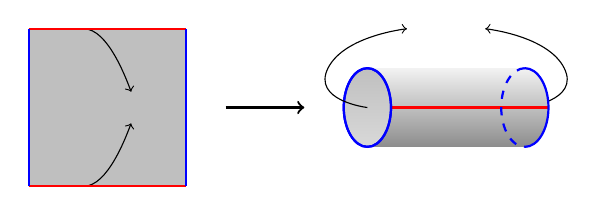
\begin{tikzpicture}
        \begin{scope}
          \fill [thick, gray!50!white] (-1, -1) rectangle (1, 1);
          \draw [->] (-0.3, 1) parabola (0.3, 0.2);
          \draw [->] (-0.3, -1) parabola (0.3, -0.2);
          \draw [thick, red] (-1, -1) -- (1, -1);
          \draw [thick, red] (-1, 1) -- (1, 1);
          \draw [thick, blue] (-1, -1) -- (-1, 1);
          \draw [thick, blue] (1, -1) -- (1, 1);
        \end{scope}

        \draw [thick, ->] (1.5, 0) -- (2.5, 0);
        \begin{scope}[shift={(4.3, 0)}]
          \draw plot [smooth, tension=1.5] coordinates {(1, 0) (1.5, 0.5) (0.5, 1)};
          \shade [bottom color=gray!90!white, top color = gray!10!white] (-1, 0.5) arc (90:-90:0.3 and 0.5) -- (1, -0.5) arc (-90:90:0.3 and 0.5) -- cycle;
          \shade [bottom color=gray!30!white, top color = gray!50!white] (-1, 0) circle [x radius = 0.3, y radius = 0.5];
          \draw [thick, red] (-0.7, 0) -- (1.3, 0);
          \draw [thick, blue] (-1, 0) circle [x radius = 0.3, y radius = 0.5];
          \draw [thick, blue] (-1, 0.5) arc (90:-90:0.3 and 0.5);
          \draw [thick, blue] (1, -0.5) arc (-90:90:0.3 and 0.5);
          \draw [thick, blue] (-1, 0.5) arc (90:270:0.3 and 0.5);
          \draw [dashed, thick, blue] (1, 0.5) arc (90:270:0.3 and 0.5);
          \draw plot [smooth, tension=1.5] coordinates {(-1, 0) (-1.5, 0.5) (-0.5, 1)};
          \draw [->] (-0.51, 1) -- (-0.5, 1);
          \draw [->] (0.51, 1) -- (0.5, 1);
        \end{scope}
      \end{tikzpicture}
    \end{center}
    Similarly, $T^3 = [0, 1]^3/{\sim}$, where the equivalence is analogous to above.
  \end{itemize}
\end{eg}
Note that even if $X$ is Hausdorff, $X/{\sim}$ may not be! For example, $\R/\Q$ is not Hausdorff.
\section{Connectivity}
Finally we can get to something more interesting. In this chapter, we will study the connectivity of spaces. Intuitively, we would want to say that a space is ``connected'' if it is one-piece. For example, $\R$ is connected, while $\R \setminus \{0\}$ is not. We will come up with two different definitions of connectivity - normal connectivity and path connectivity, where the latter implies the former, but not the other way round.

\subsection{Connectivity}
We will first look at normal connectivity.
\begin{defi}[Connected space]
  A topological space $X$ is \emph{disconnected} if $X$ can be written as $A\cup B$, where $A$ and $B$ are disjoint, non-empty open subsets of $X$. We say $A$ and $B$ \emph{disconnect} $X$.

  A space is \emph{connected} if it is not disconnected.
\end{defi}
Note that being connected is a property of a \emph{space}, not a subset. When we say ``$A$ is a connected subset of $X$'', it means $A$ is connected with the subspace topology inherited from $X$.

Being (dis)connected is a \emph{topological} property, i.e.\ if $X$ is (dis)connected, and $X\simeq Y$, then $Y$ is (dis)connected. To show this, let $f: X\to Y$ be the homeomorphism. By definition, $A$ is open in $X$ iff $f(A)$ is open in $Y$. So $A$ and $B$ disconnect $X$ iff $f(A)$ and $f(B)$ disconnect $Y$.

\begin{eg}\leavevmode
  \begin{itemize}
    \item If $X$ has the coarse topology, it is connected.
    \item If $X$ has the discrete topology and at least 2 elements, it is disconnected.
    \item Let $X\subseteq \R$. If there is some $\alpha \in \R\setminus X$ such that there is some $a, b\in X$ with $a < \alpha < b$, then $X$ is disconnected. In particular, $X\cap (-\infty, \alpha)$ and $X\cap (\alpha, \infty)$ disconnect $X$.

      For example, $(0, 1)\cup (1, 2)$ is disconnected ($\alpha = 1$).
  \end{itemize}
\end{eg}

We can also characterize connectivity in terms of continuous functions:
\begin{prop}
  $X$ is disconnected iff there exists a continuous surjective $f: X\to \{0, 1\}$ with the discrete topology.

  Alternatively, $X$ is connected iff any continuous map $f: X \to \{0, 1\}$ is constant.
\end{prop}

\begin{proof}
  $(\Rightarrow)$ If $A$ and $B$ disconnect $X$, define
  \[
    f(x) =
    \begin{cases}
      0 & x\in A\\
      1 & x\in B
    \end{cases}
  \]
  Then $f^{-1}(\emptyset)$, $f^{-1}(\{0, 1\}) = X$, $f^{-1}(\{0\}) = A$ and $f^{-1}(\{1\}) = B$ are all open. So $f$ is continuous. Also, since $A, B$ are non-empty, $f$ is surjective.

  $(\Leftarrow)$ Given $f: X\mapsto \{0, 1\}$ surjective and continuous, define $A = f^{-1}(\{0\})$, $B = f^{-1}(\{1\})$. Then $A$ and $B$ disconnect $X$.
\end{proof}

\begin{thm}
  $[0, 1]$ is connected.
\end{thm}

Note that $\Q\cap [0, 1]$ is \emph{dis}connected, since we can pick our favorite irrational number $a$, and then $\{x: x < a\}$ and $\{x: x > a\}$ disconnect the interval. So we better use something special about $[0, 1]$.

The key property of $\R$ is that every non-empty $A\subseteq [0, 1]$ has a supremum.
\begin{proof}
  Suppose $A$ and $B$ disconnect $[0, 1]$. wlog, assume $1\in B$. Since $A$ is non-empty, $\alpha = \sup A$ exists. Then either
  \begin{itemize}
    \item $\alpha \in A$. Then $\alpha < 1$, since $1 \in B$. Since $A$ is open, $\exists \varepsilon > 0$ with $B_\varepsilon(\alpha) \subseteq A$. So $\alpha + \frac{\varepsilon}{2} \in A$, contradicting supremality of $\alpha$; or

    \item $\alpha \not\in A$. Then $\alpha \in B$. Since $B$ is open, $\exists \varepsilon > 0$ such that $B_\varepsilon (\alpha) \subseteq B$. Then $a \leq \alpha - \varepsilon$ for all $a\in A$. This contradicts $\alpha$ being the \emph{least} upper bound of $A$.
  \end{itemize}

  Either option gives a contradiction. So $A$ and $B$ cannot exist and $[0, 1]$ is connected.
\end{proof}

To conclude the section, we will prove the intermediate value property. The key proposition needed is the following.
\begin{prop}
  If $f: X\to Y$ is continuous and $X$ is connected, then $\im f$ is also connected.
\end{prop}

\begin{proof}
  Suppose $A$ and $B$ disconnect $\im f$. We will show that $f^{-1}(A)$ and $f^{-1}(B)$ disconnect $X$.

  Since $A, B\subseteq \im f$ are open, we know that $A = \im f\cap A'$ and $B = \im f\cap B'$ for some $A', B'$ open in $Y$. Then $f^{-1}(A) = f^{-1}(A')$ and $f^{-1}(B) = f^{-1}(B')$ are open in $X$.

  Since $A, B$ are non-empty, $f^{-1}(A)$ and $f^{-1}(B)$ are non-empty. Also, $f^{-1}(A) \cap f^{-1}(B) = f^{-1}(A\cap B) = f^{-1}(\emptyset) = \emptyset$. Finally, $A\cup B = \im f$. So $f^{-1}(A)\cup f^{-1}(B) = f^{-1}(A\cup B) = X$.

  So $f^{-1}(A)$ and $f^{-1}(B)$ disconnect $X$, contradicting our hypothesis. So $\im f$ is connected.
\end{proof}
Alternatively, if $\im f$ is not connected, let $g: \im f \to \{0, 1\}$ be continuous surjective. Then $g\circ f: X \to \{0, 1\}$ is continuous surjective. Contradiction.

\begin{thm}[Intermediate value theorem]
  Suppose $f: X\to \R$ is continuous and $X$ is connected. If $\exists x_0, x_1$ such that $f(x_0) < 0 < f(x_1)$, then $\exists x\in X$ with $f(x) = 0$.
\end{thm}

\begin{proof}
  Suppose no such $x$ exists. Then $0\not\in \im f$ while $0 > f(x_0) \in \im f$, $0 < f(x_1) \in \im f$. Then $\im f$ is disconnected (from our previous example), contradicting $X$ being connected.
\end{proof}
Alternatively, if $f(x) \not= 0$ for all $x$, then $\frac{f(x)}{|f(x)|}$ is a continuous surjection from $X$ to $\{-1, +1\}$, which is a contradiction.

\begin{cor}
  If $f: [0, 1] \to \R$ is continuous with $f(0) < 0 < f(1)$, then $\exists x\in [0, 1]$ with $f(x) = 0$.
\end{cor}
Is the converse of the intermediate value theorem true? If $X$ is disconnected, can we find a function $g$ that doesn't satisfy the intermediate value property?

The answer is yes. Since $X$ is disconnected, let $f: X\to \{0, 1\}$ be continuous. Then let $g(x) = f(x) - \frac{1}{2}$. Then $g$ is continuous but doesn't satisfy the intermediate value property.

\subsection{Path connectivity}
The other notion of connectivity is \emph{path connectivity}. A space is path connected if we can join any two points with a path. First, we need a definition of a path.

\begin{defi}[Path]
  Let $X$ be a topological space, and $x_0, x_1 \in X$. Then a \emph{path} from $x_0$ to $x_1$ is a continuous function $\gamma: [0, 1] \mapsto X$ such that $\gamma(0) = x_0$, $\gamma(1) = x_1$.
\end{defi}

\begin{defi}[Path connectivity]
  A topological space $X$ is \emph{path connected} if for all points $x_0, x_1 \in X$, there is a path from $x_0$ to $x_1$.
\end{defi}

\begin{eg}\leavevmode
  \begin{enumerate}
    \item $(a, b), [a, b), (a, b], \R$ are all path connected (using paths given by linear functions).
    \item $\R^n$ is path connected (e.g.\ $\gamma (t) = t \mathbf{x}_1 + (1 - t)\mathbf{x}_0$).
    \item $\R^n\setminus \{0\}$ is path-connected for $n > 1$ (the paths are either line segments or bent line segments to get around the hole).
  \end{enumerate}
\end{eg}

Path connectivity is a stronger condition than connectivity, in the sense that
\begin{prop}
  If $X$ is path connected, then $X$ is connected.
\end{prop}

\begin{proof}
  Let $X$ be path connected, and let $f: X \to \{0, 1\}$ be a continuous function. We want to show that $f$ is constant.

  Let $x, y \in X$. By path connectedness, there is a map $\gamma: [0, 1] \to X$ such that $\gamma(0) = x$ and $\gamma(1) = y$. Composing with $f$ gives a map $f \circ \gamma: [0, 1] \to \{0, 1\}$. Since $[0, 1]$ is connected, this must be constant. In particular, $f(\gamma(0)) = f(\gamma(1))$, i.e.\ $f(x) = f(y)$. Since $x, y$ were arbitrary, we know $f$ is constant.
\end{proof}

We can use connectivity to distinguish spaces. Apart from the obvious ``$X$ is connected while $Y$ is not'', we can also try to remove points and see what happens. We will need the following lemma:
\begin{lemma}
  Suppose $f: X\to Y$ is a homeomorphism and $A\subseteq X$, then $f|_A: A\to f(A)$ is a homeomorphism.
\end{lemma}

\begin{proof}
  Since $f$ is a bijection, $f|_A$ is a bijection. If $U\subseteq f(A)$ is open, then $U = f(A) \cap U'$ for some $U'$ open in $Y$. So $f|_A^{-1}(U) = f^{-1}(U')\cap A$ is open in $A$. So $f|_A$ is continuous. Similarly, we can show that $(f|_A)^{-1}$ is continuous.
\end{proof}

\begin{eg} $[0, 1] \not\simeq (0, 1)$. Suppose it were. Let $f: [0, 1]$ be a homeomorphism. Let $A = (0, 1]$. Then $f|_A: (0, 1] \to (0, 1)\setminus\{f(0)\}$ is a homeomorphism. But $(0, 1]$ is connected while $(0, 1)\setminus \{f(0)\}$ is disconnected. Contradiction.

Similarly, $[0, 1)\not\simeq [0, 1]$ and $[0, 1)\not\simeq (0, 1)$. Also, $\R^n\not \simeq \R$ for $n > 1$, and $S^1$ is not homeomorphic to any subset of $\R$.
\end{eg}

\subsubsection{Higher connectivity*}
We were able to use path connectivity to determine that $\R$ is not homeomorphic to $\R^n$ for $n > 1$. If we want to distinguish general $\R^n$ and $\R^m$, we will need to generalize the idea of path connectivity to higher connectivity.

To do so, we have to formulate path connectivity in a different way. Recall that $S^0 = \{-1, 1\} \simeq \{0, 1\}\subseteq \R$, while $D^1 = [-1, 1] \simeq [0, 1] \subseteq \R$. Then we can formulate path connectivity as: $X$ is path-connected iff any continuous $f: S^0\to X$ extends to a continuous $\gamma: D^1 \to X$ with $\gamma|_{S^0} = f$.

This is much more easily generalized:
\begin{defi}[$n$-connectedness]
  $X$ is $n$\emph{-connected} if for any $k \leq n$, any continuous $f: S^k \to X$ extends to a continuous $F: D^{k + 1}\to X$ such that $F|_{S^k} = f$.
\end{defi}
For any point $p\in \R^n$, $\R^n \setminus \{p\}$ is $m$-connected iff $m \leq n - 2$. So $\R^n\setminus\{p\} \not\simeq \R^m\setminus\{q\}$ unless $n = m$. So $\R^n \not\simeq \R^m$.

Unfortunately, we have not yet proven that $\R^n \not\simeq \R^m$. We casually stated that $\R^n \setminus \{p\}$ is $m$-connected iff $m \leq n - 2$. However, while this intuitively makes sense, it is in fact very difficult to prove. To actually prove this, we will need tools from algebraic topology.

\subsection{Components}
If a space is disconnected, we could divide the space into different \emph{components}, each of which is (maximally) connected. This is what we will investigate in this section. Of course, we would have a different notion of ``components'' for each type of connectivity. We will first start with path connectivity.

\subsubsection{Path components}
Defining path components (i.e.\ components with respect to path connectedness) is relatively easy. To do so, we need the following lemma.

\begin{lemma}
  Define $x\sim y$ if there is a path from $x$ to $y$ in $X$. Then $\sim$ is an equivalence relation.
\end{lemma}

\begin{proof}\leavevmode
  \begin{enumerate}
    \item For any $x\in X$, let $\gamma_x: [0, 1] \to X$ be $\gamma(t) = x$, the constant path. Then this is a path from $x$ to $x$. So $x\sim x$.
    \item If $\gamma: [0, 1] \to X$ is a path from $x$ to $y$, then $\bar \gamma: [0, 1] \to X$ by $t \mapsto \gamma(1 - t)$ is a path from $y$ to $x$. So $x\sim y \Rightarrow y\sim x$.
    \item If $\gamma_1$ is a path from $x$ to $y$ and $\gamma_2$ is a path from $y$ to $z$, then $\gamma_2*\gamma_1$ defined by
      \[
        t\mapsto
        \begin{cases}
          \gamma_1(2t) & t\in [0, 1/2]\\
          \gamma_2(2t - 1) & t\in [1/2, 1]
        \end{cases}
      \]
      is a path from $x$ to $z$. So $x\sim y, y\sim z \Rightarrow x\sim z$.\qedhere
  \end{enumerate}
\end{proof}

With this lemma, we can immediately define the path components:
\begin{defi}[Path components]
  Equivalence classes of the relation ``$x\sim y$ if there is a path from $x$ to $y$'' are \emph{path components} of $X$.
\end{defi}

\subsubsection{Connected components}
Defining connected components (i.e.\ components with respect to regular connectivity) is slightly more involved. The key proposition we need is as follows:

\begin{prop}
  Suppose $Y_\alpha\subseteq X$ is connected for all $\alpha\in T$ and that $\bigcap_{\alpha\in T}Y_\alpha \not= \emptyset$. Then $Y = \bigcup_{\alpha\in T}Y_\alpha$ is connected.
\end{prop}

\begin{proof}
  Suppose the contrary that $A$ and $B$ disconnect $Y$. Then $A$ and $B$ are open in $Y$. So $A = Y\cap A'$ and $B = Y\cap B'$, where $A', B'$ are open in $X$. For any fixed $\alpha$, let
  \[
    A_\alpha = Y_\alpha \cap A = Y_\alpha \cap A',\quad B_\alpha = Y_\alpha\cap B = Y_\alpha \cap B'.
  \]
  Then they are open in $Y_\alpha$. Since $Y = A\cup B$, we have
  \[
    Y_\alpha = Y\cap Y_\alpha = (A\cup B)\cap Y_\alpha = A_\alpha \cup B_\alpha.
  \]
  Since $A\cap B = \emptyset$, we have
  \[
    A_\alpha \cap B_\alpha = Y_\alpha \cap (A\cap B) = \emptyset.
  \]
  So $A_\alpha, B_\alpha$ are disjoint. So $Y_\alpha$ is connected but is the disjoint union of open subsets $A_\alpha, B_\alpha$.

  By definition of connectivity, this can only happen if $A_\alpha = \emptyset$ or $B_\alpha = \emptyset$.

  However, by assumption, $\displaystyle\bigcap_{\alpha \in T}Y_\alpha \not= \emptyset$. So pick $\displaystyle y\in \bigcap_{\alpha\in T}Y_\alpha$. Since $y\in Y$, either $y\in A$ or $y\in B$. wlog, assume $y\in A$. Then $y\in Y_\alpha$ for all $\alpha$ implies that $y\in A_\alpha$ for all $\alpha$. So $A_\alpha$ is non-empty for all $\alpha$. So $B_\alpha$ is empty for all $\alpha$. So $B = \emptyset$.

  So $A$ and $B$ did not disconnect $Y$ after all. Contradiction.
\end{proof}

Using this lemma, we can define connected components:

\begin{defi}[Connected component]
  If $x\in X$, define
  \[
    \mathcal{C}(x) = \{A\subseteq X: x\in A\text{ and }A\text{ is connected}\}.
  \]
  Then $\displaystyle C(x) = \bigcup_{A\in \mathcal{C}(x)} A$ is the \emph{connected component} of $x$.
\end{defi}
$C(x)$ is the largest connected subset of $X$ containing $x$. To show this, we first note that $\{x\}\in \mathcal{C}(x)$. So $x\in C(x)$. To show that it is connected, just note that $x\in \bigcap_{A\in \mathcal{C}(x)}A$. So $\bigcap_{A\in \mathcal{C}(x)}A$ is non-empty. By our previous proposition, this implies that $C(x)$ is connected.

\begin{lemma}
  If $y\in C(x)$, then $C(y) = C(x)$.
\end{lemma}

\begin{proof}
  Since $y\in C(x)$ and $C(x)$ is connected, $C(x) \subseteq C(y)$. So $x\in C(y)$. Then $C(y)\subseteq C(x)$. So $C(x) = C(y)$.
\end{proof}

It follows that $x\sim y$ if $x \in C(y)$ is an equivalence relation and the connected components of $X$ are the equivalence classes.

\begin{eg}\leavevmode
  \begin{itemize}
    \item Let $X = (-\infty, 0) \cup (0, \infty)\subseteq \R$. Then the connected components are $(-\infty, 0)$ and $(0, \infty)$, which are also the path components.
    \item Let $X = \Q\subseteq \R$. Then $C(x) = \{x\}$ for all $x\in X$. In this case, we say $X$ is totally disconnected.
  \end{itemize}
\end{eg}
Note that $C(x)$ and $X\setminus C(x)$ need not disconnect $X$, even though it is the case in our first example. For this, we must need $C(x)$ and $X\setminus C(x)$ to be open as well. For example, in Example 2, $C(x) = \{x\}$ is not open.

It is also important to note that path components need not be equal to the connected components, as illustrated by the following example. However, since path connected spaces are connected, the path component containing $x$ must be a subset of $C(x)$.

\begin{eg}
  Let $Y = \{(0, y): y\in \R\}\subseteq \R^2$ be the $y$ axis.

  Let $Z = \{(x, \frac{1}{x}\sin \frac{1}{x}): x\in (0, \infty)\}$.
  \begin{center}
    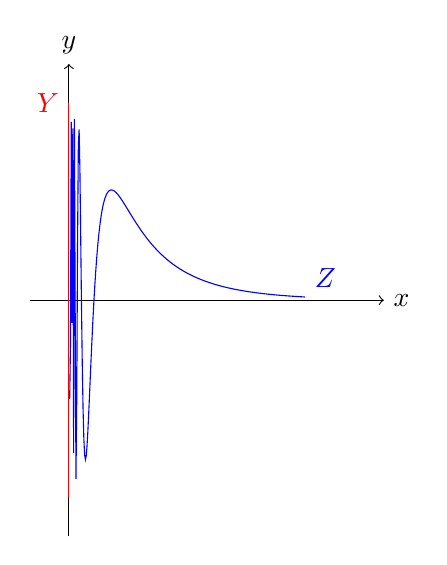
\begin{tikzpicture}
      \draw [->] (-0.5, 0) -- (4, 0) node [right] {$x$};
      \draw [->] (0, -3) -- (0, 3) node [above] {$y$};

      \draw [red] (0, -2.5) -- (0, 2.5) node [left] {$Y$};

      \draw [blue, domain=0.01:3, samples=300] plot (\x, {2.5 * exp(-\x) * sin(1 / \x r)}) node [anchor = south west] {$Z$};
    \end{tikzpicture}
  \end{center}
  Let $X = Y\cup Z\subseteq \R^2$. We claim that $Y$ and $Z$ are the path components of $X$. Since $Y$ and $Z$ are individually path connected, it suffices to show that there is no continuous $\gamma: [0, 1]\to X$ with $\gamma(0) = (0, 0)$, $\gamma(1) = (1,\sin 1)$.

  Suppose $\gamma$ existed. Then the function $\pi_2\circ \gamma: [0, 1] \to \R$ projecting the path to the $y$ direction is continuous. So it is bounded. Let $M$ be such that $\pi_2\circ \gamma (t) \leq M$ for all $t\in [0, 1]$. Let $W = X\cap (\R \times (-\infty, M])$ be the part of $X$ that lies below $y = M$. Then $\im \gamma \subseteq W$.

  However, $W$ is disconnected: pick $t_0$ with $\frac{1}{t_0} \sin\frac{1}{t_0} > M$. Then $W \cap ((-\infty, t_0)\times \R)$ and $W\cap ((t_0, \infty)\times \R)$ disconnect $W$. This is a contradiction, since $\gamma$ is continuous and $[0, 1]$ is connected.

  We also claim that $X$ is connected: suppose $A$ and $B$ disconnect $X$. Then since $Y$ and $Z$ are connected, either $Y\subseteq A$ or $Y\subseteq B$; $Z\subseteq A$ or $Z\subseteq B$. If both $Y\subseteq A, Z\subseteq A$, then $B=\emptyset$, which is not possible.

  So wlog assume $A = Y$, $B = Z$. This is also impossible, since $Y$ is not open in $X$ as it is not a union of balls (any open ball containing a point in $Y$ will also contain a point in $Z$). Hence $X$ must be connected.
\end{eg}

Finally, recall that we showed that path-connected subsets are connected. While the converse is not true in general, there are special cases where it is true.
\begin{prop}
  If $U\subseteq \R^n$ is open and connected, then it is path-connected.
\end{prop}

\begin{proof}
  Let $A$ be a path component of $U$. We first show that $A$ is open.

  Let $a\in A$. Since $U$ is open, $\exists \varepsilon > 0$ such that $B_\varepsilon(a) \subseteq U$. We know that $B_\varepsilon(a) \simeq \Int(D^n)$ is path-connected (e.g.\ use line segments connecting the points). Since $A$ is a path component and $a\in A$, we must have $B_\varepsilon(a) \subseteq A$. So $A$ is an open subset of $U$.

  Now suppose $b\in U\setminus A$. Then since $U$ is open, $\exists \varepsilon > 0$ such that $B_\varepsilon(b) \subseteq U$. Since $B_\varepsilon(b)$ is path-connected, so if $B_\varepsilon(b) \cap A \not= \emptyset$, then $B_\varepsilon(b)\subseteq A$. But this implies $b\in A$, which is a contradiction. So $B_\varepsilon(b) \cap A = \emptyset$. So $B_\varepsilon(b) \subseteq U\setminus A$. Then $U\setminus A$ is open.

  So $A, U\setminus A$ are disjoint open subsets of $U$. Since $U$ is connected, we must have $U\setminus A$ empty (since $A$ is not). So $U = A$ is path-connected.
\end{proof}

\section{Compactness}
Compactness is an important concept in topology. It can be viewed as a generalization of being ``closed and bounded'' in $\R$. Alternatively, it can also be viewed as a generalization of being finite. Compact sets tend to have a lot of really nice properties. For example, if $X$ is compact and $f: X \to \R$ is continuous, then $f$ is bounded and attains its bound.

There are two different definitions of compactness - one based on open covers (which we will come to shortly), and the other based on sequences. In metric spaces, these two definitions are equal. However, in general topological spaces, these notions can be different. The first is just known as ``compactness'' and the second is known as ``sequential compactness''.

The actual definition of compactness is rather weird and unintuitive, since it is an idea we haven't seen before. To quote Qiaochu Yuan's math.stackexchange answer (\url{http://math.stackexchange.com/a/371949}),

\begin{quotation}
  The following story may or may not be helpful. Suppose you live in a world where there are two types of animals: Foos, which are red and short, and Bars, which are blue and tall. Naturally, in your language, the word for Foo over time has come to refer to things which are red and short, and the word for Bar over time has come to refer to things which are blue and tall. (Your language doesn't have separate words for red, short, blue, and tall.)

  One day a friend of yours tells you excitedly that he has discovered a new animal. ``What is it like?'' you ask him. He says, ``well, it's sort of Foo, but\ldots''

  The reason he says it's sort of Foo is that it's short. However, it's not red. But your language doesn't yet have a word for ``short,'' so he has to introduce a new word --- maybe ``compact''\ldots

  \separator

  The situation with compactness is sort of like the above. It turns out that finiteness, which you think of as one concept (in the same way that you think of ``Foo'' as one concept above), is really two concepts: \textbf{discreteness} and \textbf{compactness}. You've never seen these concepts separated before, though. When people say that compactness is like finiteness, they mean that compactness captures part of what it means to be finite in the same way that shortness captures part of what it means to be Foo.

  But in some sense you've never encountered the notion of compactness by itself before, isolated from the notion of discreteness (in the same way that above you've never encountered the notion of shortness by itself before, isolated from the notion of redness). This is just a new concept and you will to some extent just have to deal with it on its own terms until you get comfortable with it.
\end{quotation}

\subsection{Compactness}
\begin{defi}[Open cover]
  Let $\cU\subseteq \P(X)$ be a topology on $X$. An \emph{open cover} of $X$ is a subset $\mathcal{V}\subseteq \cU$ such that
  \[
    \bigcup_{V\in \mathcal{V}} V = X.
  \]
  We say $\mathcal{V}$ \emph{covers} $X$.

  If $\mathcal{V}'\subseteq \mathcal{V}$, and $\mathcal{V}'$ covers $X$, then we say $\mathcal{V}'$ is a \emph{subcover} of $\mathcal{V}$.
\end{defi}

\begin{defi}[Compact space]
  A topological space $X$ is \emph{compact} if every open cover $\mathcal{V}$ of $X$ has a finite subcover $\mathcal{V}' = \{V_1, \cdots, V_n\} \subseteq \mathcal{V}$.
\end{defi}
Note that some people (especially algebraic geometers) call this notion ``quasi-compact'', and reserve the name ``compact'' for ``quasi-compact and Hausdorff''. We will not adapt this notion.

\begin{eg}\leavevmode
  \begin{enumerate}
    \item If $X$ is finite, then $\P(X)$ is finite. So any open cover of $X$ is finite. So $X$ is compact.
    \item Let $X = \R$ and $\mathcal{V} = \{(-R, R) : R\in \R, R > 0\}$. Then this is an open cover with no finite subcover. So $\R$ is not compact. Hence all open intervals are not compact since they are homeomorphic to $\R$.
    \item Let $X = [0, 1]\cap \Q$. Let
      \[
        U_n = X\setminus(\alpha - 1/n, \alpha + 1/n).
      \]
      for some irrational $\alpha$ in $(0, 1)$ (e.g.\ $\alpha = 1/\sqrt{2}$).

      Then $\bigcup_{n > 0} U_n = X$ since $\alpha$ is irrational. Then $\mathcal{V} = \{U_n: n\in \Z > 0\}$ is an open cover of $X$. Since this has no finite subcover, $X$ is not compact.
  \end{enumerate}
\end{eg}

\begin{thm}
  $[0, 1]$ is compact.
\end{thm}
Again, since this is not true for $[0, 1]\cap \Q$, we must use a special property of the reals.

\begin{proof}
  Suppose $\mathcal{V}$ is an open cover of $[0, 1]$. Let
  \[
    A = \{a\in [0, 1]: [0, a] \text{ has a finite subcover of }\mathcal{V}\}.
  \]
  First show that $A$ is non-empty. Since $\mathcal{V}$ covers $[0, 1]$, in particular, there is some $V_0$ that contains $0$. So $\{0\}$ has a finite subcover $V_0$. So $0\in A$.

  Next we note that by definition, if $0\leq b \leq a$ and $a\in A$, then $b\in A$.

  Now let $\alpha = \sup A$. Suppose $\alpha < 1$. Then $\alpha \in [0, 1]$.

  Since $\mathcal{V}$ covers $X$, let $\alpha \in V_\alpha$. Since $V_\alpha$ is open, there is some $\varepsilon$ such that $B_\varepsilon(\alpha) \subseteq V_\alpha$. By definition of $\alpha$, we must have $\alpha - \varepsilon/2\in A$. So $[0, \alpha - \varepsilon/2]$ has a finite subcover. Add $V_\alpha$ to that subcover to get a finite subcover of $[0, \alpha + \varepsilon/2]$. Contradiction (technically, it will be a finite subcover of $[0, \eta]$ for $\eta = \min(\alpha + \varepsilon/2, 1)$, in case $\alpha + \varepsilon/2$ gets too large).

  So we must have $\alpha = \sup A = 1$.

  Now we argue as before: $\exists V_1 \in \mathcal{V}$ such that $1 \in V_1$ and $\exists \varepsilon > 0$ with $(1 - \varepsilon, 1] \subseteq V_1$. Since $1 - \varepsilon \in A$, there exists a finite $\mathcal{V}' \subseteq \mathcal{V}$ which covers $[0, 1 - \varepsilon/2]$. Then $\mathcal{W} = \mathcal{V}' \cup \{V_1\}$ is a finite subcover of $\mathcal{V}$.
\end{proof}

We mentioned that compactness is a generalization of ``closed and bounded''. We will now show that compactness is indeed in some ways related to closedness.
\begin{prop}
  If $X$ is compact and $C$ is a closed subset of $X$, then $C$ is also compact.
\end{prop}
\begin{proof}
  To prove this, given an open cover of $C$, we need to find a finite subcover. To do so, we need to first convert it into an open cover of $X$. We can do so by adding $X\setminus C$, which is open since $C$ is closed. Then since $X$ is compact, we can find a finite subcover of this, which we can convert back to a finite subcover of $C$.

  Formally, suppose $\mathcal{V}$ is an open cover of $C$. Say $\mathcal{V} = \{V_\alpha: \alpha \in T\}$. For each $\alpha$, since $V_\alpha$ is open in $C$, $V_\alpha = C\cap V_\alpha'$ for some $V_\alpha'$ open in $X$. Also, since $\bigcup_{\alpha \in T}V_a = C$, we have $\bigcup_{\alpha\in T}V_\alpha' \supseteq C$.

  Since $C$ is closed, $U = X \setminus C$ is open in $X$. So $\mathcal{W} = \{V_\alpha': \alpha \in T\} \cup \{U\}$ is an open cover of $X$. Since $X$ is compact, $\mathcal{W}$ has a finite subcover $\mathcal{W}' = \{V_{\alpha_1}', \cdots, V_{\alpha_n}', U\}$ ($U$ may or may not be in there, but it doesn't matter). Now $U\cap C = \emptyset$. So $\{V_{\alpha_1},\cdots, V_{\alpha_n}\}$ is a finite subcover of $C$.
\end{proof}

The converse is not always true, but holds for Hausdorff spaces.
\begin{prop}
  Let $X$ be a Hausdorff space. If $C\subseteq X$ is compact, then $C$ is closed in $X$.
\end{prop}

\begin{proof}
  Let $U = X\setminus C$. We will show that $U$ is open.

  For any $x$, we will find a $U_x$ such that $U_x\subseteq U$ and $x\in U_x$. Then $U = \bigcup_{x\in U}U_x$ will be open since it is a union of open sets.

  To construct $U_x$, fix $x\in U$. Since $X$ is Hausdorff, for each $y\in C$, $\exists U_{xy}, W_{xy}$ open neighbourhoods of $x$ and $y$ respectively with $U_{xy}\cap W_{xy} = \emptyset$.
  \begin{center}
    \begin{tikzpicture}
      \draw [fill=gray!50!white] circle [radius = 1];
      \draw (-1.5, -1.5) rectangle (3, 1.5);

      \draw [red, fill=red!50!yellow, opacity=0.3] (0.8, 0) circle [radius=0.7];
      \node [red] at (0.8, 0.7) [above] {$W_{xy}$};
      \draw [red, fill=red!50!yellow, opacity=0.5] (2.2, 0.1) circle [radius=0.5];
      \node [red] at (2.2, 0.6) [above] {$U_{xy}$};

      \node at (0, 1) [below] {$C$};
      \node [circ] at (2, 0) {};
      \node at (2, 0) [right] {$x$};

      \node [circ] at (0.7, 0.1) {};
      \node at (0.7, 0.1) [right] {$y$};

    \end{tikzpicture}
  \end{center}
  Then $\mathcal{W} = \{W_{xy}\cap C: y\in C\}$ is an open cover of $C$. Since $C$ is compact, there exists a finite subcover $\mathcal{W}' = \{W_{xy_1}\cap C, \cdots, W_{xy_n}\cap C\}$.

  Let $U_x = \bigcap_{i = 1}^n U_{xy_i}$. Then $U_x$ is open since it is a finite intersection of open sets. To show $U_x \subseteq U$, note that $W_x = \bigcup_{i = 1}^n W_{xy_i} \supseteq C$ since $\{W_{xy_i}\cap C\}$ is an open cover. We also have $W_x \cap U_x = \emptyset$. So $U_x \subseteq U$. So done.
  \begin{center}
    \begin{tikzpicture}
      \draw [fill=gray!50!white] circle [radius = 1];
      \draw (-1.5, -1.5) rectangle (3, 1.5);

      \draw [red, fill=red!50!yellow, opacity=0.3] (0.8, 0) circle [radius=0.7];
      \draw [red, fill=red!50!yellow, opacity=0.5] (2.2, 0.1) circle [radius=0.5];

      \draw [blue, fill=red!50!blue, opacity=0.3] (-0.1, 0.3) circle [radius=0.9];
      \draw [blue, fill=red!50!blue, opacity=0.5] (1.7, 0) circle [radius=0.4];

      \draw [green, fill=green!50!blue, opacity=0.3] (-0.2, -0.4) circle [radius=1];
      \draw [green, fill=green!50!blue, opacity=0.5] (2, -0.2) circle [radius=0.4];

      \draw [red!50!black, thick] (0.709137, 0.694078) arc (25.97:185.97:0.9) arc (142.67:342.63:1) arc (266.27:457.46:0.7) node [anchor = south west] {$W_x$};

      \draw [blue!50!black, thick] (2.04817, 0.197101) arc (83.08:138.34:0.4) arc (183.91:237.96:0.5) arc (305.94:389.51:0.4) node [above] {$U_x$};
      \node at (0, 1) [below] {$C$};
      \node [circ] at (2, 0) {};
      \node at (2, 0) [right] {$x$};

    \end{tikzpicture}
  \end{center}
\end{proof}

After relating compactness to closedness, we will relate it to boundedness. First we need to define boundedness for general metric spaces.
\begin{defi}[Bounded metric space]
  A metric space $(X, d)$ is \emph{bounded} if there exists $M\in \R$ such that $d(x, y) \leq M$ for all $x, y\in X$.
\end{defi}

\begin{eg}
  $A\subseteq \R$ is bounded iff $A\subseteq [-N, N]$ for some $N\in \R$.
\end{eg}
Note that being bounded is \emph{not} a topological property. For example, $(0, 1)\simeq \R$ but $(0, 1)$ is bounded while $\R$ is not. It depends on the metric $d$, not just the topology it induces.

\begin{prop}
  A compact metric space $(X, d)$ is bounded.
\end{prop}

\begin{proof}
  Pick $x\in X$. Then $V = \{B_r(x): r\in \R^+\}$ is an open cover of $X$. Since $X$ is compact, there is a finite subcover $\{B_{r_1}(x), \cdots, B_{r_n}(x)\}$.

  Let $R = \max\{r_1, \cdots, r_n\}$. Then $d(x, y) < R$ for all $y\in X$. So for all $y, z\in X$,
  \[
    d(y, z) \leq d(y, x) + d(x, z) < 2R
  \]
  So $X$ is bounded.
\end{proof}

\begin{thm}[Heine-Borel]
  $C\subseteq \R$ is compact iff $C$ is closed and bounded.
\end{thm}

\begin{proof}
   Since $\R$ is a metric space (hence Hausdorff), $C$ is also a metric space.

  So if $C$ is compact, $C$ is closed in $\R$, and $C$ is bounded, by our previous two propositions.

  Conversely, if $C$ is closed and bounded, then $C\subseteq [-N, N]$ for some $N\in \R$. Since $[-N, N] \simeq [0, 1]$ is compact, and $C = C\cap [-N, N]$ is closed in $[-N, N]$, $C$ is compact.
\end{proof}

\begin{cor}
  If $A\subseteq \R$ is compact, $\exists \alpha \in A$ such that $\alpha \geq a$ for all $a\in A$.
\end{cor}

\begin{proof}
  Since $A$ is compact, it is bounded. Let $\alpha = \sup A$. Then by definition, $\alpha \geq a$ for all $a\in A$. So it is enough to show that $\alpha \in A$.

  Suppose $\alpha \not\in A$. Then $\alpha \in \R \setminus A$. Since $A$ is compact, it is closed in $\R$. So $\R \setminus A$ is open. So $\exists \varepsilon > 0$ such that $B_\varepsilon(\alpha) \subseteq \R\setminus A$, which implies that $a \leq \alpha - \varepsilon$ for all $a\in A$. This contradicts the assumption that $\alpha = \sup A$. So we can conclude $\alpha\in A$.
\end{proof}

We call $\alpha = \max A$ the maximum element of $A$.

We have previously proved that if $X$ is connected and $f: X\to Y$, then $\im f\subseteq Y$ is connected. The same statement is true for compactness.
\begin{prop}
  If $f: X \to Y$ is continuous and $X$ is compact, then $\im f \subseteq Y$ is also compact.
\end{prop}

\begin{proof}
  Suppose $\mathcal{V} = \{V_\alpha: \alpha \in T\}$ is an open cover of $\im f$. Since $V_\alpha$ is open in $\im f$, we have $V_\alpha = \im f\cap V_\alpha'$, where $V_\alpha'$ is open in $Y$. Then
  \[
    W_\alpha = f^{-1}(V_\alpha) = f^{-1}(V_\alpha')
  \]
  is open in $X$. If $x\in X$ then $f(x)$ is in $V_\alpha$ for some $\alpha$, so $x\in W_\alpha$. Thus $\mathcal{W} = \{W_\alpha: \alpha \in T\}$ is an open cover of $X$.

  Since $X$ is compact, there's a finite subcover $\{W_{\alpha_1}, \cdots, W_{\alpha_n}\}$ of $\mathcal{W}$.

  Since $V_\alpha \subseteq \im f$, $f(W_\alpha) = f(f^{-1}(V_\alpha)) = V_\alpha$. So
  \[
    \{V_{\alpha_1}, \cdots, V_{\alpha_n}\}
  \]
  is a finite subcover of $\mathcal{V}$.
\end{proof}

\begin{thm}[Maximum value theorem]
  If $f: X \to \R$ is continuous and $X$ is compact, then $\exists x\in X$ such that $f(x) \geq f(y)$ for all $y\in X$.
\end{thm}

\begin{proof}
  Since $X$ is compact, $\im f$ is compact. Let $\alpha = \max \{\im f\}$. Then $\alpha \in \im f$. So $\exists x\in X$ with $f(x) = \alpha$. Then by definition $f(x) \geq f(y)$ for all $y\in X$.
\end{proof}

\begin{cor}
  If $f: [0, 1] \to \R$ is continuous, then $\exists x\in [0, 1]$ such that $f(x) \geq f(y)$ for all $y\in [0, 1]$
\end{cor}

\begin{proof}
  $[0, 1]$ is compact.
\end{proof}

\subsection{Products and quotients}
\subsubsection{Products}
Recall the product topology on $X\times Y$. $U\subseteq X\times Y$ is open if it is a union of sets of the form $V\times W$ such that $V\subseteq X, W\subseteq Y$ are open.

The major takeaway of this section is the following theorem:
\begin{thm}
  If $X$ and $Y$ are compact, then so is $X\times Y$.
\end{thm}

\begin{proof}
  First consider the special type of open cover $\mathcal{V}$ of $X\times Y$ such that every $U\in \mathcal{V}$ has the form $U = V\times W$, where $V\subseteq X$ and $W\subseteq Y$ are open.

  For every $(x, y) \in X\times Y$, there is $U_{xy}\in \mathcal{V}$ with $(x, y)\in U_{xy}$. Write
  \[
    U_{xy} = V_{xy}\times W_{xy},
  \]
  where $V_{xy}\subseteq X$, $W_{xy}\subseteq Y$ are open, $x\in V_{xy}, y\in W_{xy}$.

  Fix $x\in X$. Then $\mathcal{W}_x = \{W_{xy}: y\in Y\}$ is an open cover of $Y$. Since $Y$ is compact, there is a finite subcover $\{W_{xy_1}, \cdots, W_{xy_n}\}$.

  Then $V_x = \bigcap_{i = 1}^n V_{xy_i}$ is a finite intersection of open sets. So $V_x$ is open in $X$. Moreover, $\mathcal{V}_x = \{U_{xy_1},\cdots , U_{xy_n}\}$ covers $V_x \times Y$.
  \begin{center}
    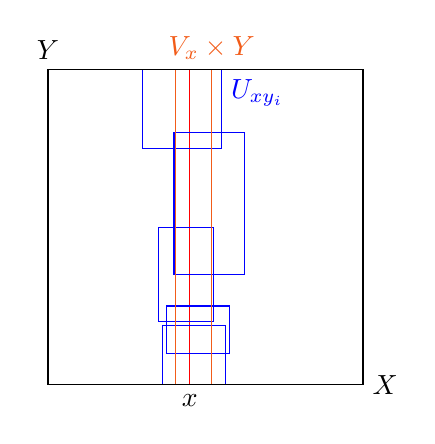
\begin{tikzpicture}
      \draw [red] (1.8, 0) node [black, below] {$x$} -- (1.8, 4);
      \draw [blue] (1.45, 0) rectangle (2.25, 0.75);
      \draw [blue] (1.5, 0.4) rectangle (2.3, 1);
      \draw [blue] (1.4, 0.8) rectangle (2.1, 2);
      \draw [blue] (1.6, 1.4) rectangle (2.5, 3.2);
      \draw [blue] (1.2, 3) rectangle (2.2, 4) node [anchor = north west] {$U_{xy_i}$};

      \draw [yellow!30!red] (1.62, 0) rectangle (2.08, 4) node [above] {$V_x\times Y$};
      \draw (0, 0) rectangle (4, 4);
      \node at (4, 0) [right] {$X$};
      \node at (0, 4) [above] {$Y$};
    \end{tikzpicture}
  \end{center}
  Now $\mathcal{O} = \{V_x: x\in X\}$ is an open cover of $X$. Since $X$ is compact, there is a finite subcover $\{V_{x_1}, \cdots, V_{x_m}\}$. Then $\mathcal{V}' = \bigcup_{i = 1}^m \mathcal{V}_{x_i}$ is a finite subset of $\mathcal{V}$, which covers all of $X\times Y$.

  In the general, case, suppose $\mathcal{V}$ is an open cover of $X\times Y$. For each $(x, y) \in X\times Y$, $\exists U_{xy}\in \mathcal{V}$ with $(x, y)\in U_{xy}$. Since $U_{xy}$ is open, $\exists V_{xy}\in X, W_{xy}\subseteq Y$ open with $V_{xy}\times W_{xy}\subseteq U_{xy}$ and $x\in V_{xy}$, $y\in W_{xy}$.

  Then $\mathcal{Q} = \{V_{xy}\times W_{xy}: (x, y)\in (X, Y)\}$ is an open cover of $X\times Y$ of the type we already considered above. So it has a finite subcover $\{V_{x_1y_1}\times W_{x_1y_1}, \cdots, V_{x_n y_n}\times W_{x_n y_n}\}$. Now $V_{x_iy_i} \times W_{x_iy_i} \subseteq U_{x_iy_i}$. So $\{U_{x_1y_1},\cdots, U_{x_n y_n}\}$ is a finite subcover of $X\times Y$.
\end{proof}

\begin{eg}
  The unit cube $[0, 1]^n = [0, 1]\times [0, 1]\times \cdots \times [0, 1]$ is compact.
\end{eg}

\begin{cor}[Heine-Borel in $\R^n$]
  $C\subseteq \R^n$ is compact iff $C$ is closed and bounded.
\end{cor}

\begin{proof}
  If $C$ is bounded, $C\subseteq [-N, N]^n$ for some $N \in \R$, which is compact. The rest of the proof is exactly the same as for $n = 1$.
\end{proof}

\subsubsection{Quotients}
It is easy to show that the quotient of a compact space is compact, since every open subset in the quotient space can be projected back to an open subset the original space. Hence we can project an open cover from the quotient space to the original space, and get a finite subcover. The details are easy to fill in.

Instead of proving the above, in this section, we will prove that compact quotients have some nice properties. We start with a handy proposition.
\begin{prop}
  Suppose $f: X\to Y$ is a continuous bijection. If $X$ is compact and $Y$ is Hausdorff, then $f$ is a homeomorphism.
\end{prop}

\begin{proof}
  We show that $f^{-1}$ is continuous. To do this, it suffices to show $(f^{-1})^{-1}(C)$ is closed in $Y$ whenever $C$ is closed in $X$. By hypothesis, $f$ is a bijection . So $(f^{-1})^{-1}(C) = f(C)$.

  Supposed $C$ is closed in $X$. Since $X$ is compact, $C$ is compact. Since $f$ is continuous, $f(C) = (\im f|_C)$ is compact. Since $Y$ is Hausdorff and $f(C) \subseteq Y$ is compact, $f(C)$ is closed.
\end{proof}

We will apply this to quotients.

Recall that if $\sim$ is an equivalence relation on $X$, $\pi: X\to X/{\sim}$ is continuous iff $f\circ \pi: X\to Y$ is continuous.

\begin{cor}
  Suppose $f: X/{\sim} \to Y$ is a bijection, $X$ is compact, $Y$ is Hausdorff, and $f\circ \pi$ is continuous, then $f$ is a homeomorphism.
\end{cor}

\begin{proof}
  Since $X$ is compact and $\pi: X\mapsto X/{\sim}$ is continuous, $\im \pi \subseteq X/{\sim}$ is compact. Since $f\circ \pi$ is continuous, $f$ is continuous. So we can apply the proposition.
\end{proof}

\begin{eg}
  Let $X = D^2$ and $A = S^1 \subseteq X$. Then $f: X/A \mapsto S^2$ by $(r, \theta) \mapsto (1, \pi r, \theta)$ in spherical coordinates is a homeomorphism.

  We can check that $f$ is a continuous bijection and $D^2$ is compact. So $X/A \simeq S^2$.
\end{eg}

\subsection{Sequential compactness}
The other definition of compactness is sequential compactness. We will not do much with it, but only prove that it is the same as compactness for metric spaces.

\begin{defi}[Sequential compactness]
  A topological space $X$ is \emph{sequentially compact} if every sequence $(x_n)$ in $X$ has a convergent subsequence (that converges to a point in $X$!).
\end{defi}

\begin{eg}
  $(0, 1) \subseteq \R$ is not sequentially compact since no subsequence of $(1/n)$ converges to any $x\in (0, 1)$.
\end{eg}

To show that sequential compactness is the same as compactness, we will first need a lemma.
\begin{lemma}
  Let $(x_n)$ be a sequence in a metric space $(X, d)$ and $x\in X$. Then $(x_n)$ has a subsequence converging to $x$ iff for every $\varepsilon > 0$, $x_n \in B_\varepsilon (x)$ for infinitely many $n$ $(*)$.
\end{lemma}

\begin{proof}
  If $(x_{n_i}) \to x$, then for every $\varepsilon$, we can find $I$ such that $i > I$ implies $x_{n_i}\in B_\varepsilon (x)$ by definition of convergence. So $(*)$ holds.

  Now suppose $(*)$ holds. We will construct a sequence $x_{n_i} \to x$ inductively. Take $n_0 = 0$. Suppose we have defined $x_{n_0}, \cdots, x_{n_{i - 1}}$.

  By hypothesis, $x_n \in B_{1/i}(x)$ for infinitely many $n$. Take $n_i$ to be smallest such $n$ with $n_i > n_{i - 1}$.

  Then $d(x_{n_i}, x) < \frac{1}{i}$ implies that $x_{n_i} \to x$.
\end{proof}

Here we will only prove that compactness implies sequential compactness, and the other direction is left as an exercise for the reader.
\begin{thm}
  If $(X, d)$ is a compact \emph{metric space}, then $X$ is sequentially compact.
\end{thm}

\begin{proof}
  Suppose $x_n$ is a sequence in $X$ with no convergent subsequence. Then for any $y\in X$, there is no subsequence converging to $y$. By lemma, there exists $\varepsilon > 0$ such that $x_n\in B_\varepsilon (y)$ for only finitely many $n$.

  Let $U_y = B_\varepsilon (y)$. Now $\mathcal{V} = \{U_y: y\in X\}$ is an open cover of $X$. Since $X$ is compact, there is a finite subcover $\{U_{y_1}, \cdots, U_{y_m}\}$. Then $x_n \in \bigcup_{i = 1}^m U_{y_i} = X$ for only finitely many $n$. This is nonsense, since $x_n \in X$ for all $n$!

  So $x_n$ must have a convergent subsequence.
\end{proof}

\begin{eg}
  Let $X = C[0, 1]$ with the topology induced $d_\infty$ (uniform norm). Let
  \[
    f_n(x) =
    \begin{cases}
      nx & x\in [0, 1/n]\\
      2 - nx & x\in [1/n, 2/n]\\
      0 & x \in [2/n, 1]
    \end{cases}
  \]
  \begin{center}
    \begin{tikzpicture}
      \draw [->] (-0.5, 0) -- (2, 0) node [right] {$x$};
      \draw [->] (0, -0.5) -- (0, 1.5) node [above] {$y$};
      \draw [red] (0, 0) -- (0.3, 1) -- (0.6, 0) -- (1.5, 0);
    \end{tikzpicture}
  \end{center}
  Then $f_n(x) \to 0$ for all $x\in [0, 1]$. We now claim that $f_n$ has no convergent subsequence.

  Suppose $f_{n_i} \to f$. Then $f_{n_i}(x) \to f(x)$ for all $x\in [0, 1]$. However, we know that $f_{n_i}(x) \to 0$ for all $x\in [0, 1]$. So $f(x) = 0$. However, $d_{\infty}(f_{n_i}, 0) = 1$. So $f_{n_i}\not \to 0$.

  It follows that $B_1(0)\subseteq X$ is not sequentially compact. So it is not compact.
\end{eg}

\subsection{Completeness}
The course ends with a small discussion about completeness. This really should belong to the chapter on metric spaces, since this is all about metric spaces. However, we put it here because the (only) proposition we have is about compactness, which was just defined recently.

Similar to what we did in Analysis, we can define Cauchy sequences.
\begin{defi}[Cauchy sequence]
  Let $(X, d)$ be a metric space. A sequence $(x_n)$ in $X$ is \emph{Cauchy} if for every $\varepsilon > 0$, $\exists N$ such that $d(x_n, x_m) < \varepsilon$ for all $n, m \geq N$.
\end{defi}

\begin{eg}\leavevmode
  \begin{enumerate}
    \item $x_n = \sum_{k = 1}^n 1/k$ is \emph{not} Cauchy.
    \item Let $X = (0, 1) \subseteq \R$ with $x_n = \frac{1}{n}$. Then this is Cauchy but does not converge.
    \item If $x_n \to x\in X$, then $x_n$ is Cauchy. The proof is the same as that in Analysis I.

    \item Let $X = \Q \subseteq \R$. Then the sequence $(2, 2.7, 2.71, 2.718, \cdots)$ is Cauchy but does not converge in $\Q$.
  \end{enumerate}
\end{eg}

Exactly analogous to what we did in Analysis, we can also define a complete space.
\begin{defi}[Complete space]
  A metric space $(X, d)$ is \emph{complete} if every Cauchy sequence in $X$ converges to a limit in $X$.
\end{defi}

\begin{eg}
  $(0, 1)$ and $\Q$ are not complete.
\end{eg}

\begin{prop}
  If $X$ is a compact metric space, then $X$ is complete.
\end{prop}

\begin{proof}
  Let $x_n$ be a Cauchy sequence in $X$. Since $X$ is sequentially compact, there is a convergent subsequence $x_{n_i}\to x$. We will show that $x_n \to x$.

  Given $\varepsilon > 0$, pick $N$ such that $d(x_n, x_m) < \varepsilon/2$ for $n,m \geq N$. Pick $I$ such that $n_I \geq N$ and $d(x_{n_i}, x) < \varepsilon/2$ for all $i> I$. Then for $n \geq n_I$, $d(x_n, x) \leq d(x_n, x_{n_I}) + d(x_{n_I}, x) < \varepsilon$. So $x_n \to x$.
\end{proof}

\begin{cor}
  $\R^n$ is complete.
\end{cor}

\begin{proof}
  If $(x_n) \subseteq \R^n$ is Cauchy, then $(x_n) \subseteq \bar B_R (0) $ for some $R$, and $\bar{B}_R(0)$ is compact. So it converges.
\end{proof}

Note that completeness is not a topological property. $\R\simeq (0, 1)$ but $\R$ is complete while $(0, 1)$ is not.
\end{document}
